\documentclass{ctuthesis}

\usepackage{wrapfig}
\usepackage{array,multirow}
\usepackage{subcaption}
\usepackage{cite}
\usepackage{listings}
\usepackage{svg}
\usepackage{hyperref}
\usepackage{makecell}
\usepackage{cleveref}
\usepackage{dirtree}
\usepackage{enumitem}
\renewcommand\theadalign{bc}
\renewcommand\theadfont{\bfseries}
\renewcommand\theadgape{\Gape[4pt]}
\renewcommand\cellgape{\Gape[4pt]}
\renewcommand{\cref}[1]{\Cref{#1}}
\renewcommand{\crefrange}[1]{\Crefrange{#1}}

\def\UrlBreaks{\do\/\do-}
\usepackage{breakurl}


\providecommand{\e}[1]{\ensuremath{\times 10^{#1}}}


\ctusetup{
    xdoctype = M,
    xfaculty = F3,
    mainlanguage = english,
    titlelanguage = english,
    title-english = {Long-term person re-identification in video},
    title-czech = {Transfer learning pro klasifikaci textu},
    department-english = {Department of Cybernetics},
    author = {Martina Tichá},
    supervisor = {Ing. Jiří Čermák, Ph.D.},
    supervisor-address = {Blindspot Solutions, Praha},
    fieldofstudy-english = {Open Informatics},
	subfieldofstudy-english = {Computer vision and digital image processing},
	day = 24,
    month = 5,
    year = 2019,
    specification-file = {zadani.pdf}, 
    front-specification = true,
	keywords-czech = {zpracování přirozeného jazyka, klasifikace textu, umělá neuronová síť, strojové učení},
	keywords-english = {natural language processing, text classification, artificial neural network, machine learning, transfer learning}
}

\ctuprocess

\begin{abstract-english}
The recent developments of Language Modeling led to advances in transfer learning methods in Natural Language Processing. Language Models pretrained on large general datasets achieved state-of-the-art results in a wide range of tasks. The \textit{Universal Language Model Fine-tuning} represents an effective transfer learning method for text classification. The goal of this thesis is to further test the robustness of this method in scenarios, commonly found in real-world applications. 

\end{abstract-english}

\begin{abstract-czech}
Nedávné vývoje v jazykových modelech vedly k posunu v transfer learning metodách ve zpracování přirozeného jazyka. Jazykové modely předtrénované na rozsáhlých obecných datasetech dosahují nejlepších výsledků v celé řadě úkolů. \textit{Universal Language Model Fine-tuning} představuje efektivní transfer learning metodu pro klasifikaci texu. Cílem této práce je hlouběji otestovat robustnost této metody ve scénářích, které se běžně nacházejí při reálných aplikacích.
\end{abstract-czech}

\begin{thanks}
Most of all, I would like to thank my supervisor, Jiří Čermák, who guided me throughout writing this thesis as well as to Štěpán Kopřiva and all the great people at Blindspot.ai.

I am grateful to all my friends and family: my parents and grandparents, my sister, and my wonderful girlfriend for always supporting me.

Finally, I want to thank the following coffee roasters, which provided  me with the much-needed fuel: Pražírna, doubleshot, KK, Dos Mundos, and Coffee Source.
\end{thanks}


\begin{declaration}
I declare that the presented work was developed independently and that I have listed all sources of information used within it in accordance with the methodical instructions for observing the ethical principles in the preparation of the university theses.
\\
\\
\\
\makebox[0.8\columnwidth]{\dotfill}
\\
Pavel Janata \\
Prague, \ctufield{day}th~\monthinlanguage{title}~\ctufield{year}
\end{declaration}


\begin{document}

\maketitle

\chapter{Introduction}

The task of person re-identification in a video (person re-ID) aims to re-identify a person that has already been recorded by a camera. It has been a subject of research for many years, since information usually used for identifying a person (mainly its face) is not reliably available, due to the person's rotation or insufficient resolution of the camera.

There is a vast variety of practical applications of person re-ID systems in both commercial and law enforcement areas. Surveillance systems are nowadays widely deployed for public safety. Hence, there is a high demand on technologies that can automatically detect strange behavior patterns in frequented places with high-security risks like airports, banks or large cultural events or in areas with strong security restrictions, e.g., embassies and laboratories.

The reason why this problem is challenging is that the surveillance cameras are located in a fixed position while the recorded people are walking at various distances from the cameras. Hence, in most cases, the resolution of the video is not sufficient for recognizing details like faces. Apart from this, there are other issues like illumination changes, occlusions, pose variations or change of clothes that make person re-ID task difficult.

In the early days, the algorithms to person re-ID were based on hand-crafted features and evaluated on small data sets. In recent years, deep learning systems utilizing newly available large-scale data sets emerged.    

Most of the current approaches assume that people going across the surveillance camera have not changed their appearance significantly. This condition restricts the person re-ID to a short-term event. However, in many places, people are likely to reappear after a long period when they have, for instance, changed their clothes. For these cases, short-term person re-ID approaches that rely on the visual aspects of the recorded people do not suffice.

To overcome this issue, an approach which ignores the person's appearance needs to be used. One of the possibilities is to construct a model which focuses on the gait of the recorded people. To achieve this, we can first extract features describing the movement of the observed person from the raw videos and feed the model with the extracted features only. Another option is to use the original videos directly but to eliminate the visual features in the initial steps. 

In this thesis, we try three approaches to do so. In the first one, we transform each frame in the video sequence into silhouettes on a white background. While this approach hides information such as the color of the clothing, some information such as the shape of the clothes the persons are wearing still remains. This can possibly confuse the model once the observed identity changes their clothes. For instance, the silhouette of a person in jeans is different from the one wearing a dress. In the second approach, we locate the joints of the observed people in each frame of the video sequence and use their position in time as the only input to the model. This way, all the information except for the movement characteristics of the walking people is dropped before the training. The third method is then the combination of both previous methods. We first transform each image frame into contours, and then we mark the skeletons constructed by joints connections on the silhouette of the observed identity. This way, the model is provided with more information and can decide itself which of them to use.
\chapter{Related Work}

In this chapter, we describe the major contributions to the person re-ID problem from the early years when person re-ID was a part of the person tracking problem, until today when person re-ID itself gains significant attention among other computer vision problems. The main focus of this thesis is the long-term person re-identification. However, the vast majority of the person re-ID approaches and benchmarks so far focus on the short-term person re-ID. Since both problems are closely related, we provide an overview of methods to either of these two. At the end of this chapter, we shortly describe the current long-term person re-ID approaches.

According to Zheng et al.\cite{Zheng_past_pres_future}, the first work, where the term "person re-identification" was used, was published in 2005 by Wojciech Zajdelet et al. \cite{first_publications}. In this work, the authors describe a system enabling a mobile robot, equipped with a color vision system, to track people and to keep track of them when they leave the field of view. Later on, the re-identification task separated from person tracking problem, and the focus was put on the person retrieval in multi-camera vision systems with the goal to find identical persons in footage from different cameras.


\section{Image-based person re-ID}
The first approaches to person re-ID focused on image matching rather than matching of the whole videos.
There are two sub-tasks the person re-ID systems need to solve: 
 
\begin{enumerate}[label=(\alph*)]
\item image description  - defines the feature vector that is extracted from the raw image pixels
\item similarity metric - defined to measure the similarity between two images
\end{enumerate}

Based on how the re-ID systems handle these two sub-tasks, we will categorize them same as in \cite{Zheng_past_pres_future} into hand-crafted systems and deep-learning systems.
\subsubsection{Hand-crafted systems}

The crucial step in hand-crafted re-ID systems is the choice of features extracted from the raw input data. The data needs to be examined, and the algorithms for feature extraction are then designed based on the properties of the data. Hence, the resulting re-ID systems are often tuned for the input data and do not generalize well when used on a different data set.

Most commonly used features in the pedestrian description are low-level features such as color, texture, or gradient. For color representation, Prosser et al. \cite{re_id_by_support_vector_ranking} and many others use eight color channels - RGB, HS, and YCbCr. In the same work, 21 texture filters (Gabor \cite{gabor_filters} and Schmid \cite{schmid_filters}) were applied for the luminance channel. Texture features, on the other hand, can be represented as Local Binary Patterns (LBP) \cite{pcca}. Low-level features can further be encoded into descriptors such as color histograms, fisher vectors \cite{fisher_vectors} or Histogram of Oriented Gradients \cite{HOG_human_detection}. The spacial structure of the image can be analyzed by dividing the image into a grid or stripes and the features extracted from these separated regions \cite{pcca}.

The second core element that needs to be chosen in hand-crafted systems is the distance metric that measures the similarity between two samples. The core idea of the similarity measurement is to keep the feature vector of the same identity close while maintaining a distance between different identities. According to \cite{Zheng_past_pres_future}, the most commonly used distance metric is based on the Mahalanobis distance function, which is a generalization of the Euclidean distance metric that uses linear scaling and rotations of the feature spaces. 
\subsubsection{Deep-learning systems}

In recent years, end-to-end convolutional neural networks (CNN) have been successfully applied in many areas of computer vision \cite{DL_for_vison}. The main advantage of CNNs is their ability to automatically learn the feature representation without any explicit specification of the feature extraction technique. Currently, most of the state-of-the-art re-ID methods are based on deep-learning systems as they have significantly outperformed the previously mentioned hand-crafted systems. 

The first works in re-ID that used deep learning techniques were \cite{deep_for_re_id} and \cite{deep_filters_for_re_id}. Since then, two main approaches to person re-ID in deep learning emerged: classification  models and verification models (see \cite{Zheng_past_pres_future} for more details). 

In classification models, the training data consist of labeled images categorized into classes. The input to the neural network is then a single image of an identity which needs to be classified by the model. 

Verification models, on the other hand, take a set of images as their inputs and estimate the similarity between them. One example of the verification model is the Siamese neural networks \cite{siamese_network}. This network consists of two identical sub-networks whose outputs are connected by a joining neuron. The training data consists of pairs of samples which are labeled as either the same or different class. The network is then trained to recognize the data from the same class.

\section{Video-based person re-ID}
In recent years, due to the increasing data richness, video-based person re-ID is gaining more and more attention in research. In this case, the re-ID algorithm consumes the whole sequence of images as its input, and so the algorithm can collect more information about the appearance of each individual. Moreover, when keeping the input as a sequence, spatial-temporal features can be extracted for each identity. This way, the model gets additional information about movements. Similarly, as in image-based person re-ID systems, there are two groups of video-based person re-ID systems:
\subsubsection{Hand-crafted systems}
In 2010, Bazzani et al.\cite{multi_shot_person_reid} proposed a work where a set of images of the same individuality is condensed into a highly informative signature, which is then matched with the signature of another set of images. It shows that using multiple frames per person instead of a single image significantly improves the results of the re-ID. Such methods are usually denoted as "multi-shot person re-ID". The disadvantage of the multi-shot strategy is that it does not incorporate any temporal cues in the model. In 2014, Wang et al. \cite{video_ranking_re-id} proposed a method that automatically selects the most discriminative video segment from a noisy image sequence. Space-time features are then extracted from this segment. In \cite{fisher_composition_for_video_reid}, the video sequences are first decomposed into sequences of individual body units, from which Fisher vectors are extracted and combined into a descriptor of the whole video sequence. Gao at al. \cite{temporally_aligned_pooling} proposes a method that uses the periodicity property of pedestrians of the "best" walking cycle from noisy motion information. To describe the video data in the selected walking cycle, the cycle is first divided into several segments. Each segment is then described by temporally aligned pooling.  
\subsubsection{Deep-learning systems}
In video-based re-ID deep-learning systems, in order to utilize the spatial-temporal features, the neural network is usually constructed so that it takes the whole sequence of images as its input. There are two prevailing approaches to achieve this. Pooling based methods aggregate appearance features (e.g., CNN, color, LBP) extracted from individual images into a vector representing the whole video sequence \cite{MARS}. The main disadvantage of this method is that it cannot model well the temporal changes in human pose. The second popular method for video-based re-ID utilizes the schema of recurrent neural networks (RNN), which are special types of a neural network that can aggregate both image-level features and human dynamics information. In \cite{recurrent_feature_aggregation_lstm}, a special type of RNN called Long Short-Term Memory (LSTM) is fed with low-level features extracted from individual frames of input video sequences. The outputs of several such LSTMs are then connected to a softmax layer. N. McLaughlin at al.  \cite{pooling_with_RNN} uses a convolutional neural network that incorporates a recurrent final layer which enables the features extracted from individual frames to be enriched by features from previously seen frames. The outputs from this neural network are then combined using temporal pooling, which gives an appearance feature of the whole sequence  \cite{pooling_with_RNN}. 
\section{Long-term person re-ID}
All the above-mentioned methods are based on appearance matching of the observe identities, which limits their application to a short-term person re-ID. To build a model that is able to re-identify a person after a long time when visual features like clothing are no more reliable, one needs to utilize personal characteristics that do not change by the time and that are unique for each identity. To my knowledge, the only contribution to long-term person re-ID so far is in 2018 by Zhang et al. \cite{long-term_re-id_true_motion}. In this work, partially inspired by the success of dense trajectory on action recognition \cite{action_recognition}, the authors present a model based on a hypothesis that people keep constant motion patterns under non-distraction walking condition. 

\chapter{Technical Background} \label{ch:technical_background}

In this chapter, we provide an overview of the theory, which is crucial for understanding the person re-ID approaches that will be described in the following chapters. 

We start with the description of the terms Deep learning, Artificial neuron, and describe a general artificial neural network. Later, we continue with the convolutional neural networks, recurrent neural networks, long-short term neural networks and convLSTM neural networks. We will also explain the edge extraction and joints detection methods, the we use in the data pre-processing phase in our experiments.

\section{Deep learning}\label{tb:deep_learning}
Deep learning is part of machine learning, which is based on Artificial Neural Networks \cite{DLWiki}. The idea of the Artificial Neural Networks (ANN) first emerged in the 1940s after McCulloch and Pitts introduced simplified neurons in 1943 \cite{NN_introduction}. The ANNs are inspired by the biological neural networks that are present in the brain. The reason why the ANNs are gaining much attention in the recent years is that they have been shown to outperform previous state-of-the-art techniques in several tasks and together with the increasing amount of available data in fields like computer vision, they are believed to have a great potential in the future.

\subsection{Artificial Neuron}\label{tb:ann}
The Artificial Neuron is the elementary unit of every ANN. It represents a function $f$, which process an input $\textbf{x}=[x_1, x_2, ..., x_n]$ such that
\begin{equation}
    f(\textbf{x)}=\varphi(F(\textbf{x}))= \varphi(\sum_{i=1}^{n}w_ix_i + b).
\end{equation}
In the above equation, the function $\varphi$ is a so called activation function, which decides, whether a neuron should be activated and what is its relevance. The main purpose of the activation function is to introduce non-linearity into the output of a neuron. This is important as most real-world problems are not linear and the neural networks need to be able to learn these non-linear representations. The scalars $w_1,...,w_n$ are learnable weights and scalar $b$ is a learnable bias.

The neurons in a neural network are connected by connections and the learnable weights represent the significance of this connections. Each input to a neuron consists of outputs of previous neurons that have a connection with the current neuron. Figure \ref{fig:neuron} shows a diagram of a single neuron.

\begin{figure}[h!]
    \centering
    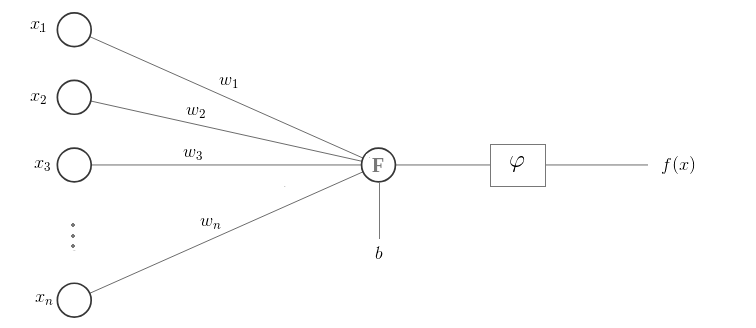
\includegraphics[scale=0.4]{figures/neuron.png}
    \caption{Neuron} 
    \label{fig:neuron}
\end{figure}

\subsection{General ANNs}\label{tb:ann}
Every ANN consists of an input layer, one or more hidden layers, and an output layer. Every layer contains multiple neurons, and they have connections to neurons from adjacent layers. In case all neurons from one layer are connected to all neurons from the previous layer, we talk about a dense (or fully connected) layer. An example of a neural network with two hidden layers can be seen in Figure \ref{fig:simple_ann}.

\begin{figure}[h!]
    \centering
    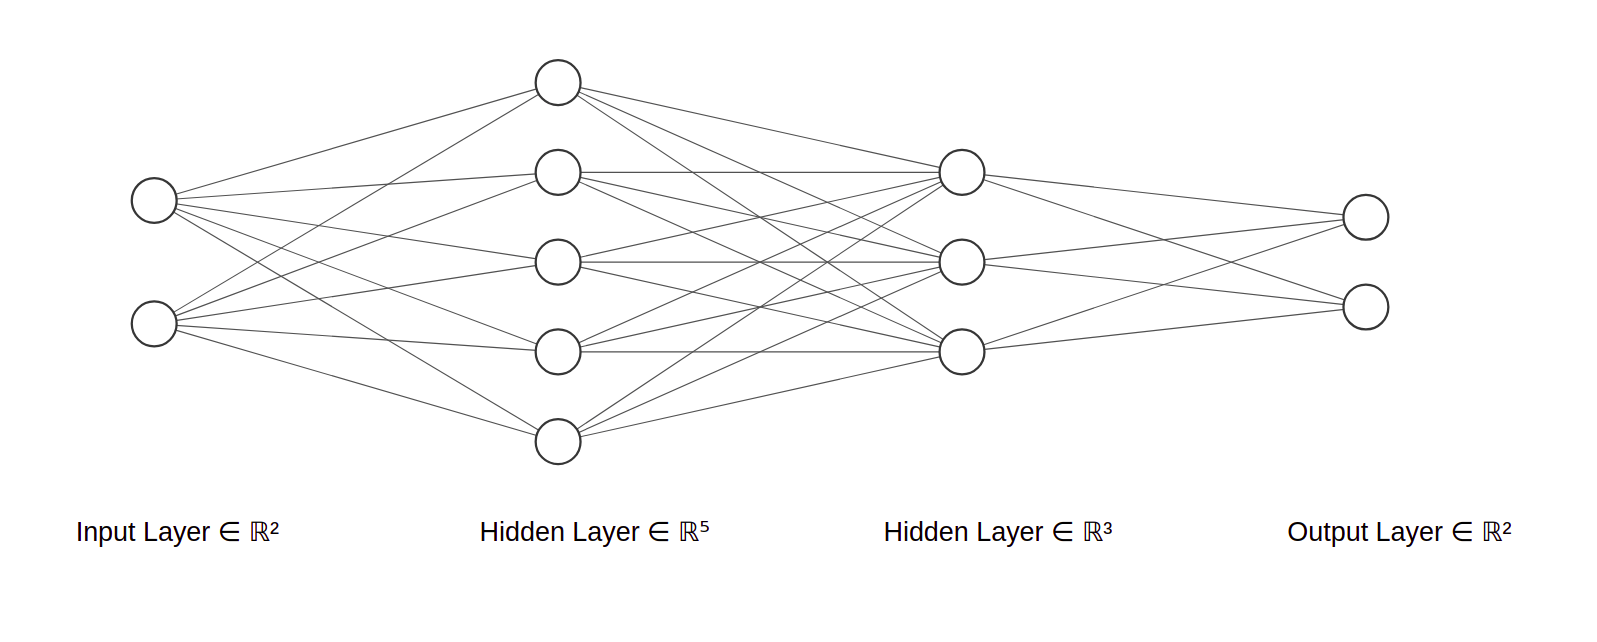
\includegraphics[scale=0.2]{figures/simple_nn.png}
    \caption{Artificial Neural Network diagram} 
    \label{fig:simple_ann}
\end{figure}

\subsection{Convolutional Neural Networks}\label{tb:cnn}
Convolutional neural networks (CNNs) are a particular type of ANNs, that were originally designed for the usage in image processing applications. The characteristics of CNNs is the usage of convolution in at least one of its layers. 

The reason why CNNs are so widely used in computer vision problems is that even small-sized images contain a tremendous amount of information. A grey-scale $620\times480$ image contains 297 600 pixels. Assuming that every pixel intensity of this image is an input to a fully-connected network, each neuron of this network requires 297 600 weights. Hence, the number of free parameters in the network becomes extremely large as the image size increases. This leads to overfitting and slow performance. In CNNs, the total number of free parameters is reduced using the convolutional layers.

Another reason for the usage of CNNs is its translation invariance. In many pattern detection tasks, the same pattern can be found in different places in the image, and it would be inefficient to train neurons to recognize the same pattern on different positions independently.

A CNN usually consists of three types of layers: convolutional layers, pooling layers, and fully connected layers.

\subsubsection{Convolutional Layers}

In the convolutional layers, every neuron represents a convolution of a filter (called kernel) and a small patch in the image. The neurons are applied along the width and height dimensions of the image. The kernels have the same depth as the images, but smaller width and height. The output width and height of each layer depend on the kernel size, number of strides (number of pixels that the kernel is shifted between each computation) and the number of zero-padding pixels around the input image. 

The main trick of the convolutional layers is the fact that the trainable weights (filters) are shared among a number of neurons in one layer. Hence, the number of free parameters in the convolutional layer is significantly lower than in a fully connected layer. The output from a convolution of the input with one filter (all neurons sharing the same weights) is called a feature map. Each filter in one layer generates one feature map, and together they make up the output depth. Every entry in the feature map can be interpreted as the output of one neuron. 

Figure \ref{fig:ConvNN} displays a mapping of a convolutionar layer. 
Every patch from the input on the left hand side (one example is highlighted by the red block) is convolved with all filters of the layer. The convolutions of all patches from the input with one filter produce one feature map (one of them is highlighted by the red plane on the right). The whole output consists of all feature maps, where the number of feature maps corresponds to the number of filters in this layer.

Every feature map detects some feature in the input. For example, in image processing, one feature map can detect horizontal edges, another one vertical edges, etc.

\begin{figure}[h!]
    \centering
    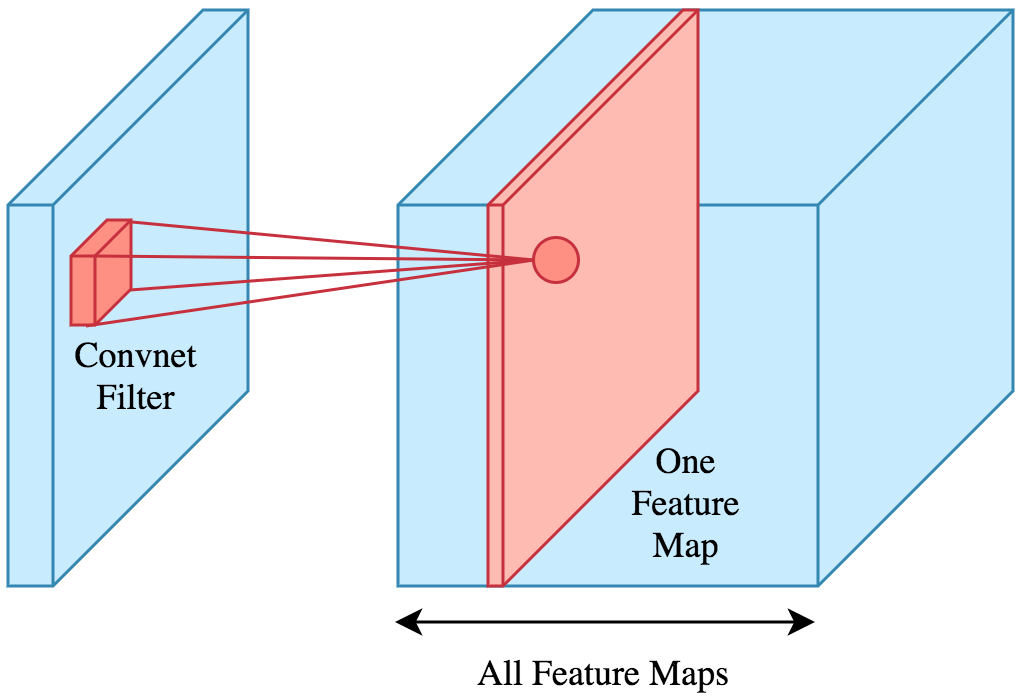
\includegraphics[scale=0.2]{figures/convNN.png}
    \caption{Convolutional layer \cite{ConvNN_layer_img}}
    \label{fig:ConvNN}
\end{figure}

\subsubsection{Pooling Layers}
The Pooling Layers progressively reduce the size of the data passed throw them, and hence, they reduce the number of parameters of the network. There are several non-linear functions which can be used for pooling. The most common one is max pooling, where the input is partitioned into rectangles from which the max value is selected. 

\begin{figure}[h!]
    \centering
    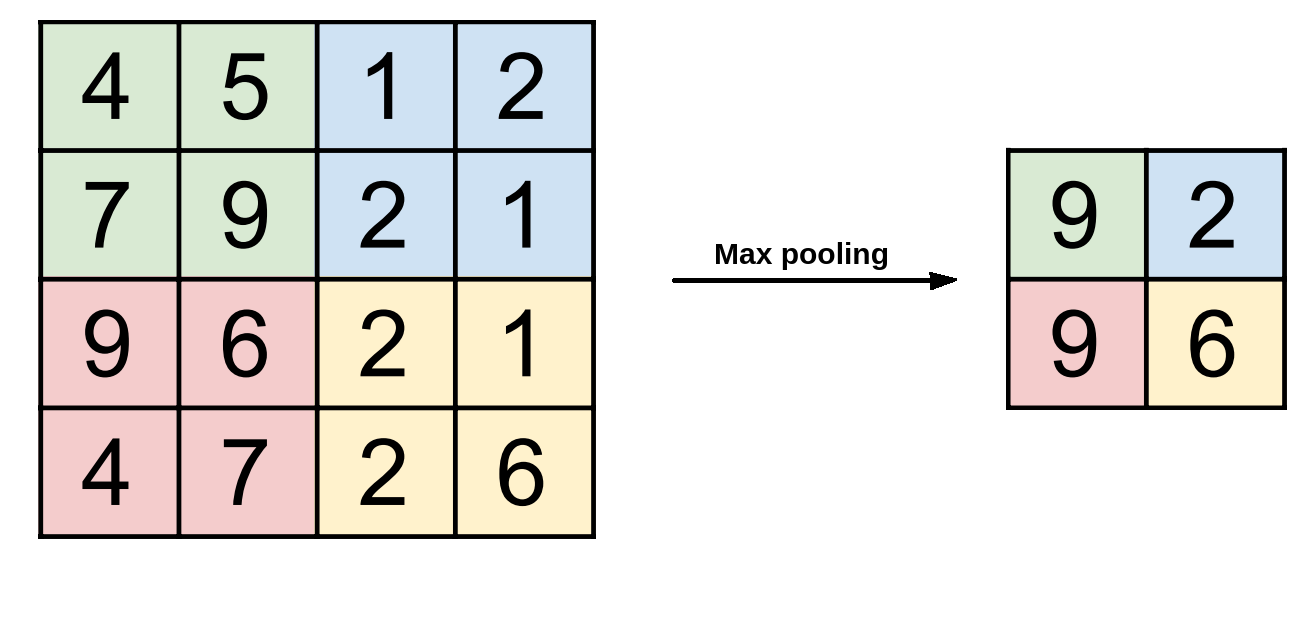
\includegraphics[scale=0.2]{figures/max_pooling.png}
    \caption{Max pooling}
    \label{fig:maxPooling}
\end{figure}

\subsubsection{Fully Connected Layers}
In the CNNs, the Fully Connected Layers are usually present at the end of the network. They are fully connected to all activations in the previous layers and perform the high-level reasoning of the network such as classification based on the features extracted by the preceding layers etc.

\begin{figure}[h!]
    \centering
    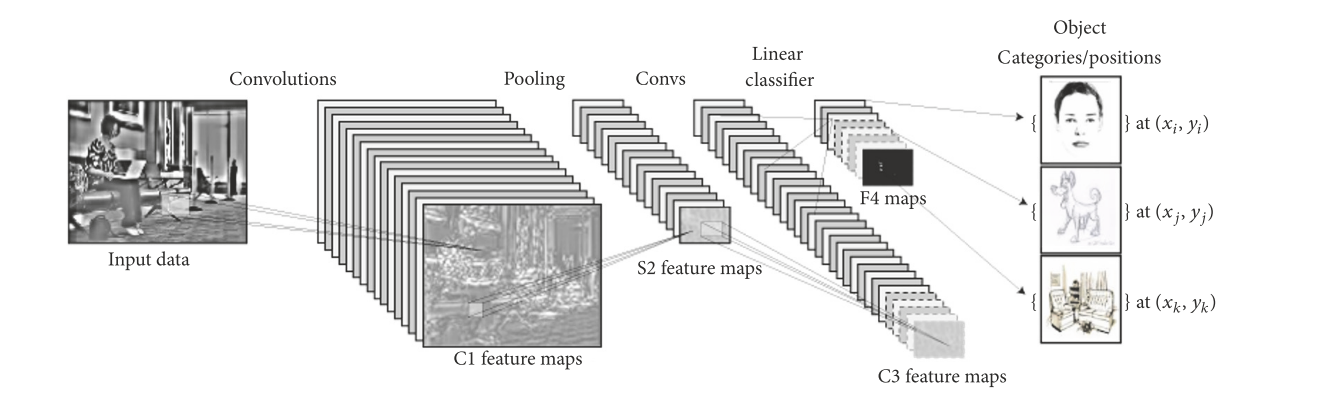
\includegraphics[scale=0.3]{figures/CNN_example.png}
    \caption{CNN architecture example \cite{DL_for_computer_Vision}}
    \label{fig:DL}
\end{figure}

\subsection{Recurrent Neural Networks}\label{tb:rnn}
The traditional feed-forward neural networks are a powerful tool with many applications. However, one of their shortcomings is that when applied on sequential data, they fail to capture the sequential structure as they are not able to reason about the output based on the previously seen outputs. This is where the Recurrent Neural Networks (RNNs) come into play. They are networks with loops in them, allowing the output to be influenced not only by the weights that are learned during the training process but also by a state vector representing the context based on previously seen inputs and outputs.

The schema of a recurrent neural network is illustrated in Figure \ref{fig:RNN}. Here, a chunk of a neural network, A, receives the input $x_t$ and produces the output $h_t$. The loop allows information to be passed from one step of the network to the next one. We can also interpret the RNN as a chain of multiple identical network models, each passing a message to the following one (see Figure \ref{fig:RNN_unrolled}).
\begin{figure}[h!]
    \centering
    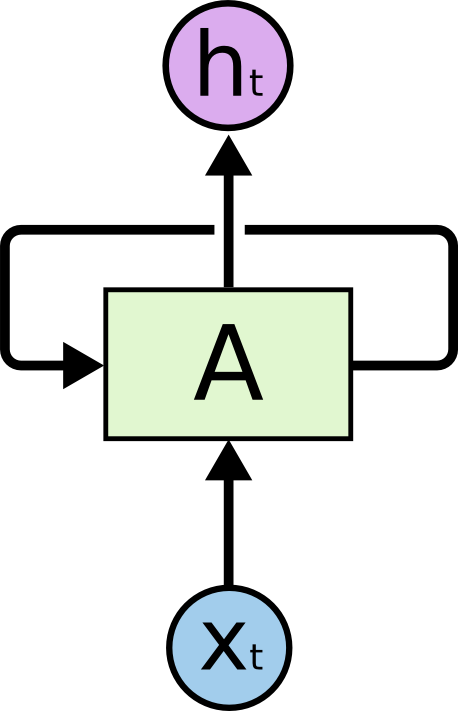
\includegraphics[scale=0.3]{figures/RNN-rolled.png}
    \caption{Recurrent neural network \cite{LSTM_blog}}
    \label{fig:RNN}
\end{figure}

\begin{figure}[h!]
    \centering
    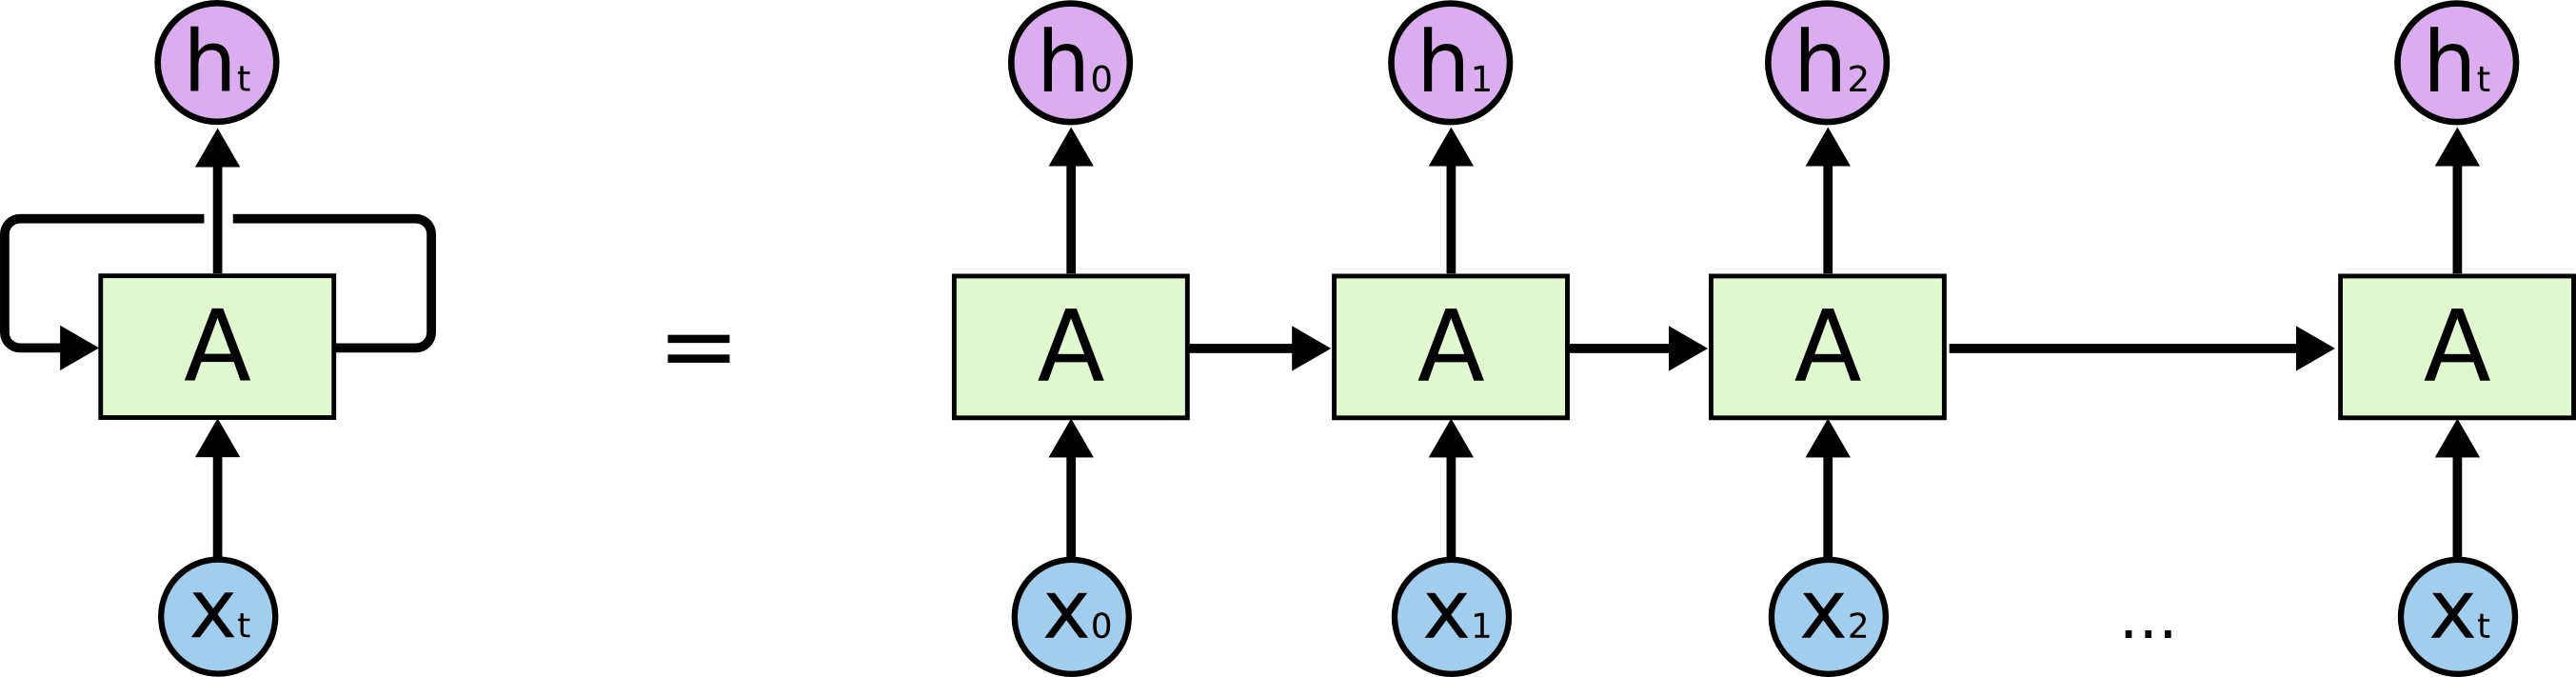
\includegraphics[scale=0.3]{figures/RNN-unrolled.png}
    \caption{Unrolled recurrent neural network \cite{LSTM_blog}}
    \label{fig:RNN_unrolled}
\end{figure}


\subsubsection{The problem of Long-Term Dependencies}

In some cases, it is enough for the network to only remember the last few outputs from a sequence for good reasoning about the newly seen input. However, there are cases where the network needs to look far in the history to be able to classify the output for a given input correctly. In the case of the standard RNNs, the repeating modules have a very simple structure. Usually, they consist of one $tanh$ layer (see Figure \ref{fig:simple_rnn}). In theory, despite their simple structure, RNNs are perfectly able to learn this so-called Long-Term Dependencies. However, in practice, they are not performing well in such situations (see \cite{RNN_long_term} for more information). To overcome this issue, in 1997, Long Short-Term Memory Neural Networks were introduced \cite{LSTM_paper}.


\begin{figure}[h!]
    \centering
    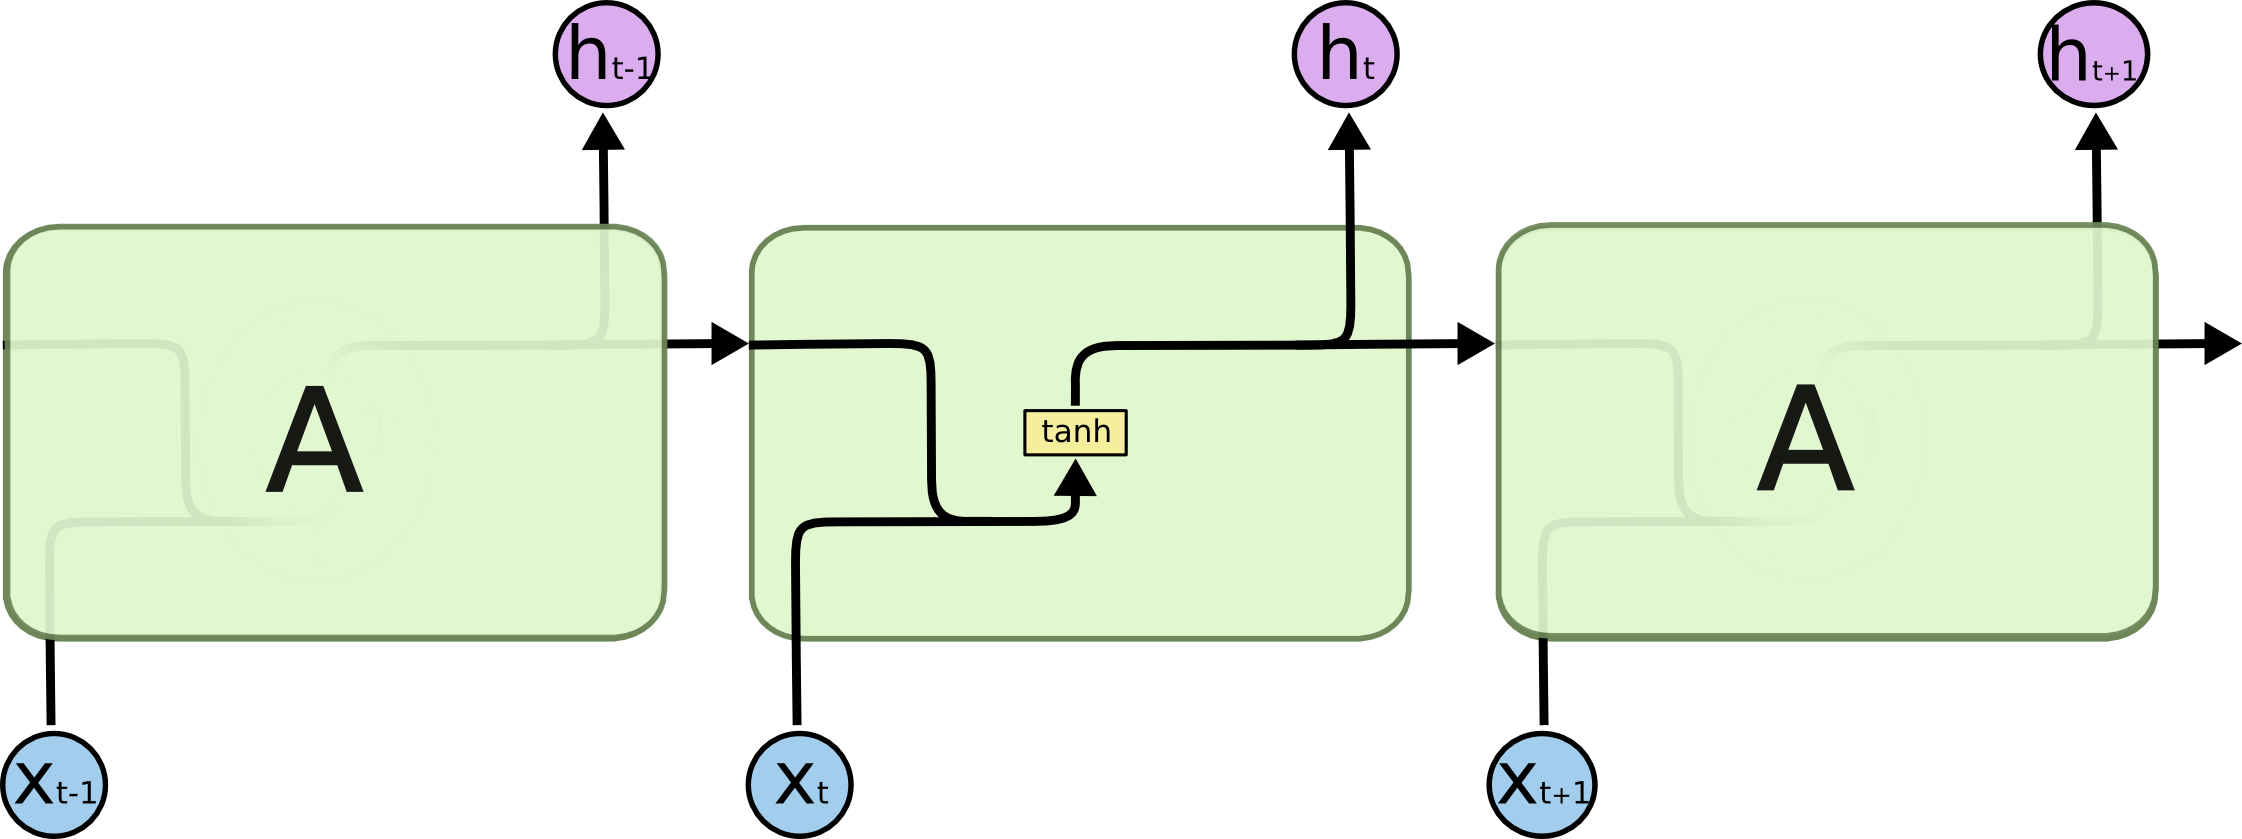
\includegraphics[scale=0.45]{figures/LSTM3-SimpleRNN.png}
    \caption{Repeating module in standard RNNs \cite{LSTM_blog}}
    \label{fig:simple_rnn}
\end{figure}


\subsection{Long Short-Term Memory Neural Networks}\label{tb:lstm}
The Long Short-Term Memory Neural Networks (LTSMs) are a special type of RNNs, which are designed to avoid the long-term dependency problem. Unlike the standard RNNs, LSTMs are able to remember information for long time periods. 


The key difference between the standard RNNs and LSTMs is the structure of the repeating network modules. Instead of having one single neural network layer, the schema of the LSTM repeating module is more complicated (see Figure \ref{fig:lstm_modes_schema}). 


\begin{figure}[h!]
    \centering
    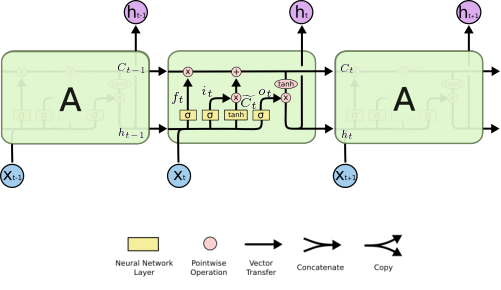
\includegraphics[scale=0.7]{figures/LSTM3-chain.png}
    \caption{Repeating module in standard LSTMs \cite{LSTM_blog}}
    \label{fig:lstm_modes_schema}
\end{figure}


It consists of two parts. The first part is the cell state (the horizontal line passing throw the pointwise addition and pointwise multiplication nodes), which can be thought of as a transporter running down the whole chain of the network models. 

The second part is composed of three so called gates and one $tanh$ layer. The gaits consist of a sigmoid layer and a pointwise multiplication operation and output a number between zero and one, which specifies how much of the component should be remembered. The $tanh$ layer, on the other hand, creates new candidate values, which can be to some extent (depending on the gates) added to the cell state.

The formulation of the LSTM module can be summarized by following equations.

\begin{align}
    f_t &=\sigma(W_{xf}\cdot x_t + W_{hf}\cdot h_{t-1} +b_f)\\
    i_t &=\sigma(W_{xi} \cdot x_t + W_{hi} \cdot h_{t-1} +b_i)\\
    \widetilde{C}_t&=tanh(W_{xC}\cdot x_t + W_{hC} \cdot h_{t-1} +b_C)\\
    C_t&=f_t\circ C_{t-1}+i_t\circ \widetilde{C_t}\\
    o_t&=\sigma(W_{xo} \cdot x_t + W_{ho} \cdot h_{t-1} +b_o)\\
    h_t&=o_t\circ tanh(C_t)
\end{align}
where $\circ$ represents a pointwise multiplication, $\cdot$ a scalar multiplication and $+$ represents a vector addition.

For detail information about the LSTMs, see \cite{LSTM_blog}. 


\subsection{ConvLSTM}\label{tb:convLstm}
We have already explained the convolutional neural networks, which are networks, that are able to learn the spacial dependencies in images, and LSTM networks, that cover the temporal dependencies. However, one might be interested in covering both the special and the temporal dimension (e.g., when processing video sequences). For this case, the Convolutiona LSTMs (convLSTMs) were designed. 

The convLSTMs follow the same structure as the LSTMs, but instead of a matrix multiplication, they use convolution operation inside of the LSTM module. Hence, the input and output data of the convLSTM are 3 dimensional vectors, unlike in the standard LSTM module where the input and output data are one-dimensional. This way, convLSTMs are able to capture the underlying spatial features. 

The formulation of the convLSTM module can be summarized by equations (3.8) throw (3.13). 

\begin{align}
    f_t &=\sigma(W_{xf}* x_t + W_{hf}* h_{t-1} +b_f)\\
    i_t &=\sigma(W_{xi} * x_t + W_{hi} * h_{t-1} +b_i)\\
    \widetilde{C}_t&=tanh(W_{xC}* x_t + W_{hC} * h_{t-1} +b_C)\\
    C_t&=f_t\circ C_{t-1}+i_t\circ \widetilde{C_t}\\
    o_t&=\sigma(W_{xo} * x_t + W_{ho} * h_{t-1} +b_o)\\
    h_t&=o_t\circ tanh(C_t)
\end{align}
where $*$ represents a convolution operation.

For more information about the convLSTMs, see \cite{convLSTM}.

\section{Edge detection}\label{tb:edge_detection}
In the edge detection problem, the task is to find edges and object boundaries in raw images. This problem is of a great importance to a variety of computer vision areas, and hence, a great number of approaches to edge detection have been developed, ranging from early developed method using the Sobel operator \cite{sobel} or Canny detector \cite{canny} to recently developed methods based on convolutional neural networks such as DeepEdge \cite{deepedge} or CSCNN \cite{cscnn}. In this thesis, we use the Holistically-Nested Edge Detection library (HED) available at \cite{xie15hed}, which provides an image-to-image method transforming the raw image into image of the objects boundaries. The method is build upon a deep learning model that leverages fully convolutional neural networks and deeply-supervised nets \cite{deeply_supervised_nets}, adopting a slightly modified VGGNet architecture \cite{vgg}. An example of the HED image transformation can be seen in Figure \ref{fig:hed}. For more information about the HED library, see \cite{xie15hed}.

\begin{figure}[h!]
    \centering
    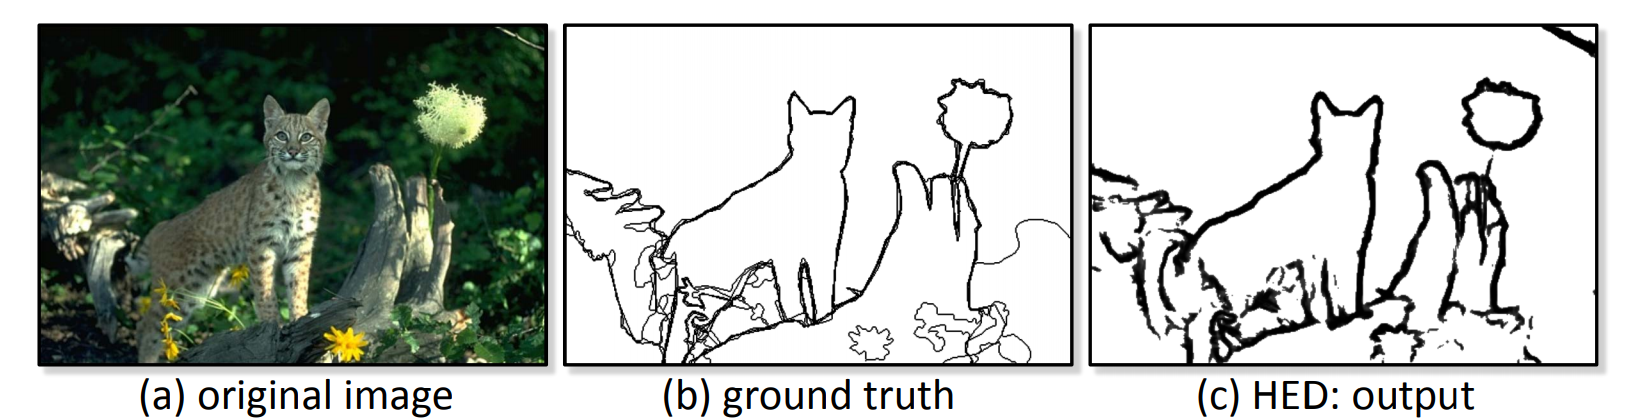
\includegraphics[scale=0.22]{figures/HED.png}
    \caption{HED edge detection example, \cite{xie15hed}}
    \label{fig:hed}
\end{figure}

\section{Skeleton extraction}\label{tb:joints_location}
The task of skeleton extraction (also known as pose estimation) consists in finding the locations of joints of people in a picture or a video and connecting the right ones so that the result forms skeletons of the people. For this purpose, we use in this thesis the Openpifpaf library available at \cite{openpifpaf}.

This library is based on the work by Sven Kreiss at al. \cite{openPifPaf_paper}. It provides a bottom-up method for multi-person 2D human pose estimation. 

The whole method is based on a ResNet \cite{resnet} network with two head networks: PIF (Part Intensity Field), which localizes the body parts, and PAF (Part Association Field) used to associate body parts with each other so that they form full human poses. The whole model is displayed in Figure \ref{fig:pifpaf}. The input is an image of size $(H, W)$ with three color channels. The neural network based encoder produces PIF and PAF fields. The decoder is then applied to convert the PIF and PAF fields into pose estimates containing 17 joints each. Each joint is represented by an $x$ and $y$ coordinate and a confidence score.

For more information, see \cite{openPifPaf_paper}.

\begin{figure}[h!]
    \centering
    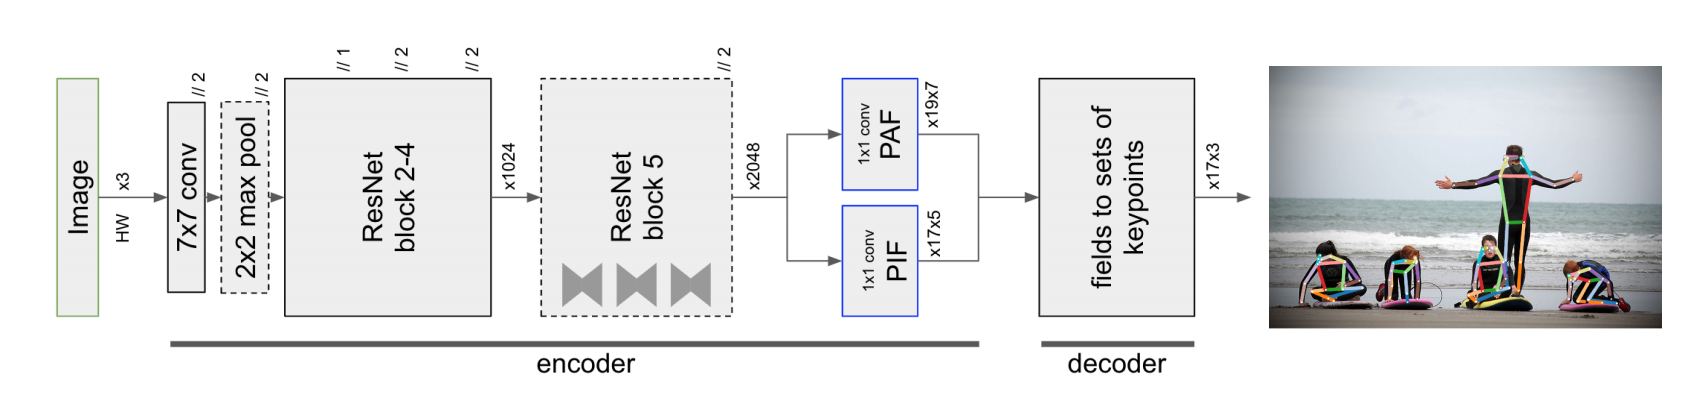
\includegraphics[scale=0.22]{figures/PifPafModel.png}
    \caption{Openpifpaf model \cite{openPifPaf_paper}}
    \label{fig:pifpaf}
\end{figure}


\chapter{Gait as a biometrics} \label{ch:gait_recognition}
In this chapter, we provide an overview of body measurements, that can be used for a person-identification. In particular, we discuss the usage of the gait as a mean of identification and describe the families of methods for gait recognition. This chapter was inspired by \cite{gafurov2007survey}.
 
\section{Biometrics}
The term Biometric refers to a metric related to some human characteristics (biometric identifier). The biometric identifiers can be divided into two groups:
\begin{itemize}
    \item Physiological identifiers (e.g., fingerprints, palm veins, DNA, iris...)
    \item Behavioral identifiers (e.g., voice, gait, typing rhythm...)
\end{itemize}
\bigbreak
There are many human traits, that can be used for the biometric identification. Jain et al. \cite{biometrics} described seven factors that should be considered when selecting a particular biometric to be used in a specific situation:
\begin{itemize}
    \item \textit{Universality} - every person possess this characteristic
    \item \textit{Uniqueness} - the characteristic is unique for each person
    \item \textit{Permanence} - the trait does not vary over time
    \item \textit{Measurability} - the measurements are easy to obtain
    \item \textit{Performance} - relates to the accuracy, speed, and robustness of the technology used 
    \item \textit{Acceptability} - the technique is accepted well by the individuals of the relevant population such that they are willing to have their biometric trait captured
    \item \textit{Circumvention} - the trait cannot be easily imitated
\end{itemize}
\bigbreak
Currently, the most popular biometric-based person identification methods are based on iris recognition, face recognition, and fingerprints recognition. These methods are, in general, very accurate, fast, and robust. However, their main disadvantage is that they either require physical contact (fingerprint scanning) or at least a cooperation of the subject (photo shooting from a short distance and a suitable angle for iris or face recognition). 

Gait, as a human trait, does not have these constraints and can easily be observed even from a distance. The studies in psychophysics \cite{friend_by_gait} show that humans can recognize people by the way they walk, which indicates the presence of identity information in their gait. According to a medical study from the year 1967 \cite{gait_total_pattern}, there are 24 different components of a human gait, and if all of them are considered, gait is unique for each person. For these reasons, the usage of gait to distinguish people is nowadays an attractive topic among researchers. 

\section{Approaches to Gait Recognition}
Based on how the information about the individual's gait is obtained, gait recognition methods can be divided into three categories.
\subsection{Wearable sensor-based gait recognition}
In the Wearable sensors-based gait recognition methods, the gait information is collected using body-worn motion recording sensors. The sensors can be fastened at different locations on the human body and can hence measure various metrics such as speed, movement frequency, the maximal and minimal distance between specific body part, etc. These methods can be, depending on the sensors, very precise in capturing the human body movements. The apparent main disadvantage, on the other hand, is the need of the sensors to be fastened onto bodies of the observed identities.
\subsection{Floor sensor-based gait recognition}
In the case of the Floor sensor-based gait recognition methods, a set of sensors is installed on the floor. These sensors enable to measure gait features such as stride length, stride cadence, or time on toe vs. time on heel ratio when a person walks on the floor. The main advantage of this method is that it does not need any cooperation from the side of the observed identities. The sensors can be installed in front of the doors of buildings and provide information about the gait of people who want to enter. On the other hand, sensors located on the floor can hardly monitor other body parts than legs and feet, and the person identification is then carried out on incomplete data.
\subsection{Machine vision-based gait recognition}
In the machine vision-based gait recognition methods, the gait is captured by a video-camera from a distance. Various processing techniques are then applied to the videos to extract gait features for recognition purpose. The main advantage of this method is that the only necessary device that needs to be installed to collect the information about the target people is a surveillance camera, which is nowadays common equipment in most of the public places. The disadvantage of this method is its computational complexity as the processing of video sequences is, in general, significantly more computationally demanding than processing signals from sensors from the previous two methods. However, thanks to the increasing power of technologies, this obstacle is becoming less and less significant, and the machine vision-based gait recognition methods are believed to have significant potential in the field of the person recognition.

\section{Challenges}
Several factors may have a negative influence on the accuracy of gait recognition methods. We can divide them into two groups.
\begin{itemize}
    \item \textit{Internal factors}. These factors change the natural gait due to some physiological changes in the body such as pregnancy, sickness, injury, gaining or losing weight, drunkenness, aging and so on. 
    \item \textit{External factors}. These factors either impose challenges to the recognition algorithm (e.g., insufficient lighting conditions, varying viewing angles or indoor vs outdoor environments) or temporary change the natural gait such as walking surface conditions (grass vs concrete, dry vs slippery floor, etc.), type of shoes (mountain shoes vs dancing shoes), objects carrying (e.g., backpack, suitcase, etc.) and so on.
\end{itemize}
\bigbreak
Due to all these factors that need to be considered and managed in order to build a robust gait recognition system, for the time being, gait cannot be considered as a replacement for traditional person identification mechanisms like fingerprints or iris-based person identification. However, there are known cases where gait analysis was used as evidence in criminal investigations. One example is the investigation of an armed robbery in 2000 in the UK \cite{forensic_gait_analys}.
\chapter{Datasets} \label{ch:data_sets}
In this chapter, we provide an overview of the publicly available datasets for the person re-ID. We then describe in details the MARS dataset, which we used in our experiments, together with the cleansing process that we applied to select the most suitable video sequences from all videos of the MARS dataset.
\section{Overview}
There are several publicly available datasets for the person re-ID. A comprehensive overview can be found in \cite{re_ID_data_overview}. One of the first was the ViPeR dataset \cite{ViPeR} released in 2007. It contains 1264 images of 632 identities. Since then, a few more small-scale datasets appeared. The first dataset large enough for deep learning was the CUHK03 \cite{cuhk03} introduced in 2014. It includes 13164 images of 1360 persons. One of the most popular person re-ID datasets is the Market-1501 dataset \cite{market_dataset} from the year 2015. It consists of 12936 images of 751 persons. This dataset was later extended into a MARS dataset \cite{MARS}, which is the first large scale video-based person re-id dataset \cite{re_ID_data_overview}. This dataset was used for our experiments, and we describe it later in this chapter in more details. To my knowledge, the biggest re-ID dataset with respect to the number of identities to date is the MSMT17 dataset \cite{MSMT17}. It consists of 4101 identities and 126441 images. This dataset, however, does not contain tracking sequences and could not have been used for our purposes.
\section{MARS Dataset}
For the purpose of this thesis, we have used the MARS dataset \cite{MARS}, which is the biggest video-based person re-ID dataset to date \cite{re_ID_data_overview}. It contains 1261 identities and 1191003 video frames from around 20715 videos. All the recorded videos come from six near-synchronized cameras in the campus of Tsinghua. An example of a video sequence consisting of seven image frames is displayed in Figure
\ref{fig:mars_example}.

\begin{figure}[h!]
    \centering
    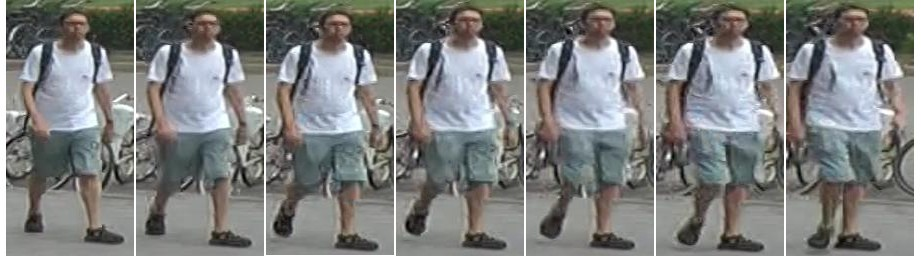
\includegraphics[scale=0.4]{figures/0006C2T0002F016_22.jpg}
    \caption{MARS data set example} 
    \label{fig:mars_example}
\end{figure}


Even though MARS dataset is a suitable dataset to be used as a training dataset for the person re-identification from video, there are some issues which have to be solved before using it for the model training. 

\subsection{Issues of the data set in re-ID}

The main problem of the raw dataset is the so called Class Imbalance Problem \cite{class_imbalance}, which in case of the MARS data set means that the number of video sequences per identity varies significantly, ranging from 1 to 271 videos. Hence, when training a classification model, the identities for which there are many video sequences in the training dataset would be prioritized by the model which would harm its generalization ability. 

Another issue is the length of the videos, which ranges from very short sequences consisting of less than five image frames up to very long sequences depicting dozens of steps of a walking person. If we want to build a model that should re-identify an identity based on the way they walk, the very short videos will not provide enough information for the model to be able to recognize them.

The third problem that needs to be mentioned when talking about the MARS dataset is the quality of the videos, which is also varying throughout the dataset. The most frequent defect of the videos is the partial occlusion, which limits the possibility to describe the movement of the whole bodies.

\subsection{Dataset cleansing} \label{dataset:cleansing}
In order to solve the previously mentioned issues, we apply the following cleansing process on the MARS dataset. We cut the original video sequences into subsequences of 20 images, which roughly corresponds to a video of two steps of a walking person. The reason why we decided for the sequences of 20 images is that even though we would extract more information about the identities from longer sequences, we would loose a lot of identities as for many of them, there is not enough data to extract sufficient amount of longer video sequences. From these short sequences, we select up to 10 sequences for each identity. The selection is based on a parameter that denotes the quality of the sequence with respect to visibility of the moving identity. This step will be further explained in Chapter \ref{ch:proposed_solutions}. Out of these ten sequences, at most 4 come from the same camera as such video sequences are very similar and would not bring any additional value for the model training. Those identities where there are less than 4 such video cuts are dropped from the data set. This way, we obtain a data set consisting of 1210 identities. The distribution of number of identities for number of videos is displayed in diagram \ref{fig:num_of_videos_per_id}.

\begin{figure}[h!]
    \centering
    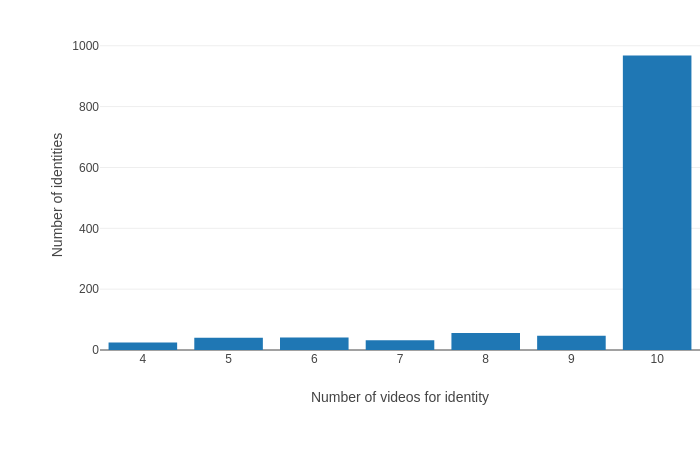
\includegraphics[scale=0.4]{figures/identities_per_num_of_videos.png}
    \caption{Distribution of number of identities for number of videos} 
    \label{fig:num_of_videos_per_id}
\end{figure}



\chapter{Proposed solutions} \label{ch:proposed_solutions}

In this thesis, we use deep learning-based methods to solve the problem of long term person re-identification. We propose three approaches: Edge-based method, Skeleton-based method, and Combined method. In all of these methods, the first step is the preprocessing of the video sequences. As each video consists of a sequence of images, we describe the preprocessing on individual image frames. The outputs of the preprocessing phase are then fed into a neural network. For the model implementation, we use the Keras library. 

\section{Edge-based method}

In the Edge-based method, the preprocessing phase consists of a transformation of the original video frames into gray-scale images depicting the edges from the original images. We use this approach to remove information about a person's clothing, which typically changes in the long-term scope. The model is therefore forced to use information about the movement and body shape of the persons to perform the re-id. The transformed videos are then fed into a neural network. 

\subsection{Edge extraction}
For the video frames transformation in the preprocessing phase of this method, we use the edge detection neural network described in  \ref{tb:edge_detection}. An example of this transformation applied on one video frame from the MARS dataset \cite{MARS} is depicted in figure \ref{fig:countour_extraction}.

\begin{figure}[h!]
    \centering
    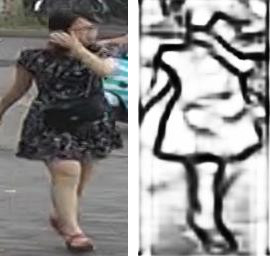
\includegraphics[scale=0.4]{figures/contours_example.jpg}
    \caption{Edge extraction example: left hand side - original image, right hand side - image after edge extraction}
    \label{fig:countour_extraction}
\end{figure}

\subsection{Neural Network description}
The structure of the neural network used in the edge-based model is illustrated in Figure \ref{fig:nnModel}. 

The first part of this neural network consists of three ConvLSTM layers (see Section \ref{tb:convLstm}), each of them followed by a batch normalization layer \cite{batch_normalization}. The input to the first ConvLSTM layer is a sequence of 20 images with the resolution of 64$\times$64 pixels. In the last ConvLSTM layer, this sequence is combined into one output, which is then fed into the second part of this network. 

The second part of the network consists of an 2D Average Pooling layer, followed by a Flatten layer and two Dense layers with ReLu and Softmax activation functions.

\begin{figure}[h!]
    \centering
    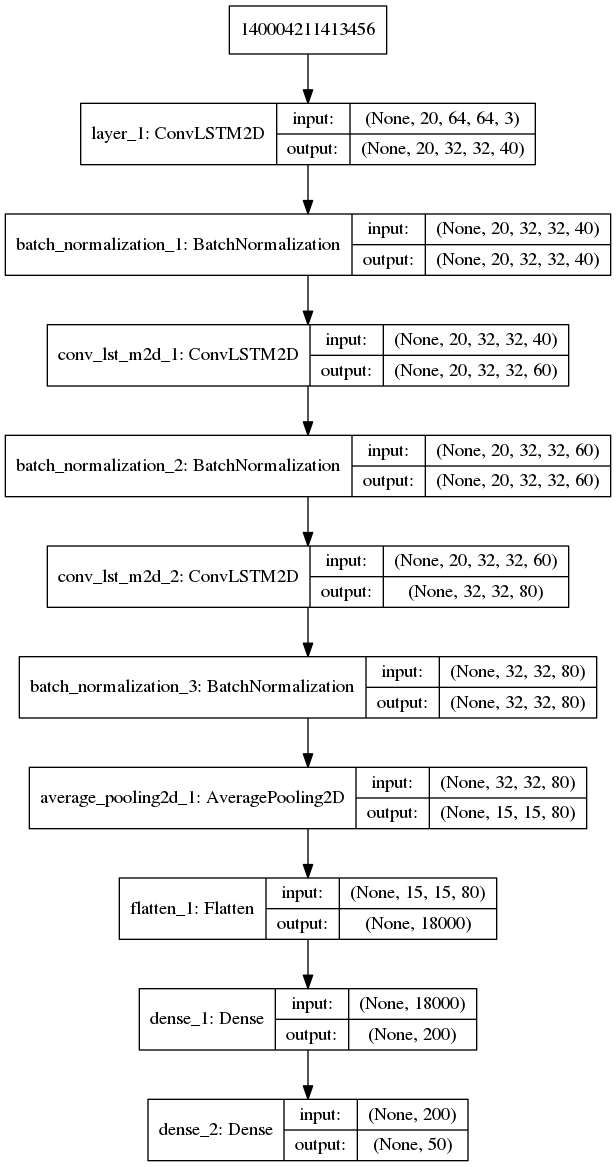
\includegraphics[scale=0.4]{figures/model.png}
    \caption{Edge based model NN}
    \label{fig:nnModel}
\end{figure}

\subsection{Weak points}

The main drawback of this method is the fact that when extracting the edges, we keep the information about the shapes of the persons. However, the shape of the moving body changes with the clothes they are wearing. Hence, the same identities can look very different in two different videos.

The second problem of this method is that when extracting the edges of the observed bodies, other people or objects remain in the images in case they were clearly visible in the original image. These undesired edges can be confusing for the model.

\section{Skeleton-based method}
In the skeleton-based method, the whole images are transformed into a list of positions of seventeen joints describing the skeleton of the body. As the person walks, the changes of positions of their joints are representing their gait. The sequence of joints locations is the only input to the model. Hence, the model does not receive any information about the person's appearance and needs to rely solely on their movements.

\subsection{Joints extraction}
The video preprocessing phase in this method consists of location and extraction of joints of the observed people in the video sequences. To achieve this, we use the openpifpaf library \cite{openpifpaf}, which provides a bottom-up method for the 2D human pose estimation. The input to the method is the image of a person for whom the pose should be estimated. The output is then the image with marks on the positions of the 17 most significant joints of this person and lines connecting this joints and highlighting the whole skeleton. There are two modes in which this methods works: single-pose estimation, which selects the most reliable person with respect to their visibility in the image and highlights the skeleton for them only, and multi-pose estimation, which estimates the pose of all identities that are visible in the picture. One example of the estimated skeleton can be seen in Figure \ref{fig:kreiss2019pifpaf}. For our purpose, we use the single-pose estimation mode as we only are focused on one person in the image and we suppose they will always be the most visible one. The openpifpaf library is based on the work \cite{kreiss2019pifpaf}.

In case of the Skeleton-based person re-id method, we do not need the whole skeletons depicted in the images, but only the positions of the 17 joints of the observed bodies. These can be easily obtained with some small modifications in the source code of the openpifpaf library. The input to such modified method for the 2D human pose estimation remains the same, the output is then a 34-dimensional vector containing the $x$ and $y$ coordinates of the 17 joints in the image. The sequences of this 34 dimensional vectors is then used as the input to the neural network described in the following section.

\begin{figure}[h!]
    \centering
    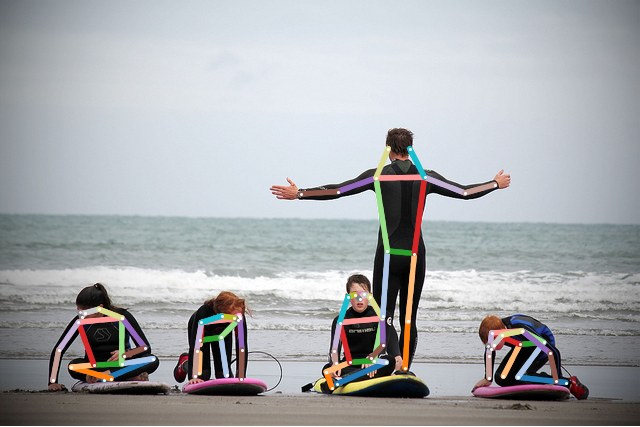
\includegraphics[scale=0.4]{figures/skeleton.png}
    \caption{Example of the human pose estimation using openpifpaf}
    \label{fig:kreiss2019pifpaf}
\end{figure}


\subsection{Neural Network description}
The structure of the neural network that we use in the skeleton based person re-id method can be seen in Figure \ref{fig:skeleton_based_model}. It can be again separated into two parts.

The first part consists of three LSTM layers (see Section \ref{tb:lstm}), each of which is followed by a batch normalization layer. The input to the first LSTM layer is a sequence of 20 34-dimensional vectors representing the $x$ and $y$ coordinates of the 17 most significant joints of the observed body (see previous section). In the last LSTM layer, the whole sequence is combined into one output, that is then fed into the second part of the network.

The second part of the network consists of two Dense layers. The first one has the ReLu activation function, and the second one is the classifying layer and uses the Softmax activation function.

\begin{figure}[h!]
    \centering
    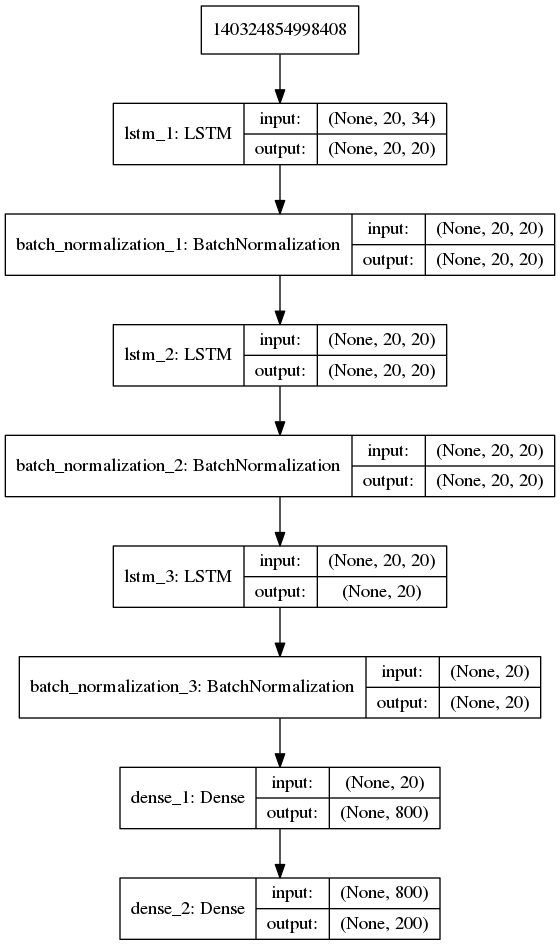
\includegraphics[scale=0.4]{figures/model_kpts.png}
    \caption{Skeleton based model NN}
    \label{fig:skeleton_based_model}
\end{figure}

\section{Combined method}
In the third method, we combine both previous approaches. First, we transform the images into edges. In the second step, we draw the skeleton onto the edges. The model is then provided with sequences of images depicting the edges together with the skeleton. This way, the model itself decides about the relevance of this two information and can combine them accordingly.

\subsection{Combining the edges with skeleton}
At this point, we already have both the edges of the observed identities in the images and the locations of their joints from the previous two methods. In order to depict the skeletons onto the transformed images, what we need to do is to draw lines connecting the adjacent joints. To keep some additional information, we draw the lines depicting hands blue, lines depicting the body green and those highlighting the legs red. An example of a seven-frame sequence with edges and skeleton drawn as described is illustrated in Figure \ref{fig:edges_with_skeleton}.

\begin{figure}[h!]
    \centering
    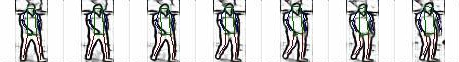
\includegraphics[scale=0.8]{figures/edges_with_skeleton.png}
    \caption{Edges with skeleton example}
    \label{fig:edges_with_skeleton}
\end{figure}

\subsection{Neural Network description}
In the combined method, as the inputs have not changed from the edges method in anything but having the additional skeleton drawn on the video frames, we use the very same neural network as in the edges method (see Figure \ref{fig:nnModel}). 

\chapter{Experiments evaluation} \label{ch:results}
In this chapter, we present the results of the experiments described in the previous chapter, together with the evaluation metrics and train and test data split used.

\section{Train and test data split}
The process of obtaining the cleansed dataset used for our experiments was described in Section \ref{dataset:cleansing}. After the cleansing process, we get a data set consisting of 1210 identities, where for each of them, there are between four and ten video sequences consisting of 20 image frames. Additionally, at most four of these sequences for one identity come from the same camera, as such sequences are too similar to bring any new information to the model if kept in a higher number. This fact also needs to be taken into account when splitting the data into train and test sets, meaning that arbitrary two sequences for one identity obtained from one camera need to be present both in either train or test set. To ensure this, we aggregate all the video sequences for all identities into groups where one group contains sequences for one identity captured by one camera. These groups are then randomly split into train and test sets. In our experiments, we use $90\%$ of the groups as the train data and $10\%$ groups remain as the test data.

\section{Evaluation metrics}
For the evaluation of our experiments, we use the standard model evaluation metrics which are loss and accuracy.

\subsubsection{Loss}
Loss is defined as the difference between the true value and the value predicted by the model. For the multi-class classification problem, the common loss function is the cross-entropy defined as

\begin{equation}
    CL(Y,\tilde{Y})=-\sum_{i=1}^{n}\sum_{j=1}^{m}y_{i,j}log(\tilde{y}_{i,j}), \: y_{i,j}\in Y, \: \tilde{y}_{i,j}\in \tilde{Y}.
\end{equation}

In the above definition, $y_{i,j}$ denotes the true value, i.e. $y_{i,j}=1$ if sample $i$ belongs to the class $j$ and $y_{i,j}=0$ otherwise, $\tilde{y}_{i,j}$ denotes the probability that sample $i$ belongs to the class $j$ predicted by the model, $Y$ is the set of all possible $y_{i,j}$ values and $\tilde{Y}$ represents the set of all probability predictions from the model $\tilde{y}_{i,j}$.

\subsubsection{Accuracy}
The accuracy of the model measures the model performance. We define it as 
\begin{equation}
    Accuracy=\frac{Number\:of\:correct\:predictions }{Total\:number\:of\:predictions}.
\end{equation}

\section{Results}
The following results were obtained from five runs of each of the methods described in Chapter \ref{ch:proposed_solutions}.  
\subsubsection{Edge-based method}
The following table provides the results of the five independent runs of the Edge-based algorithm.

\begin{figure}[h!]
    \centering
    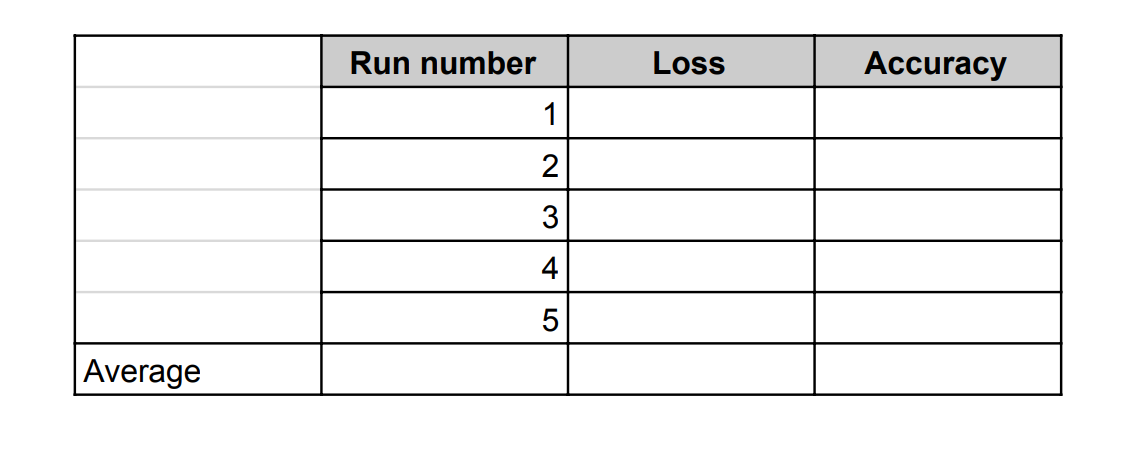
\includegraphics[scale=0.22]{figures/results.png}
    \caption{Results of five runs of the Edge-based algorithm}
    \label{fig:edge_based_met_results}
\end{figure}



Figure \ref{fig:edge_based_met_results} shows the Accuracy resp. Loss learning curve for the Edge-based method. The x-axis represents the number of iterations of the algorithm and the y-axis denotes the accuracy resp. loss.

Figure \ref{fig:missclassifications} shows an example of all  miss-classifications for one sequence. For simplicity, we only display one image frame for each sequence. On the left-hand side, we see the original image. The images on the right-hand side are then all representants of sequences wrongly classified as being of the left identity.

\begin{figure}[h!]
    \centering
    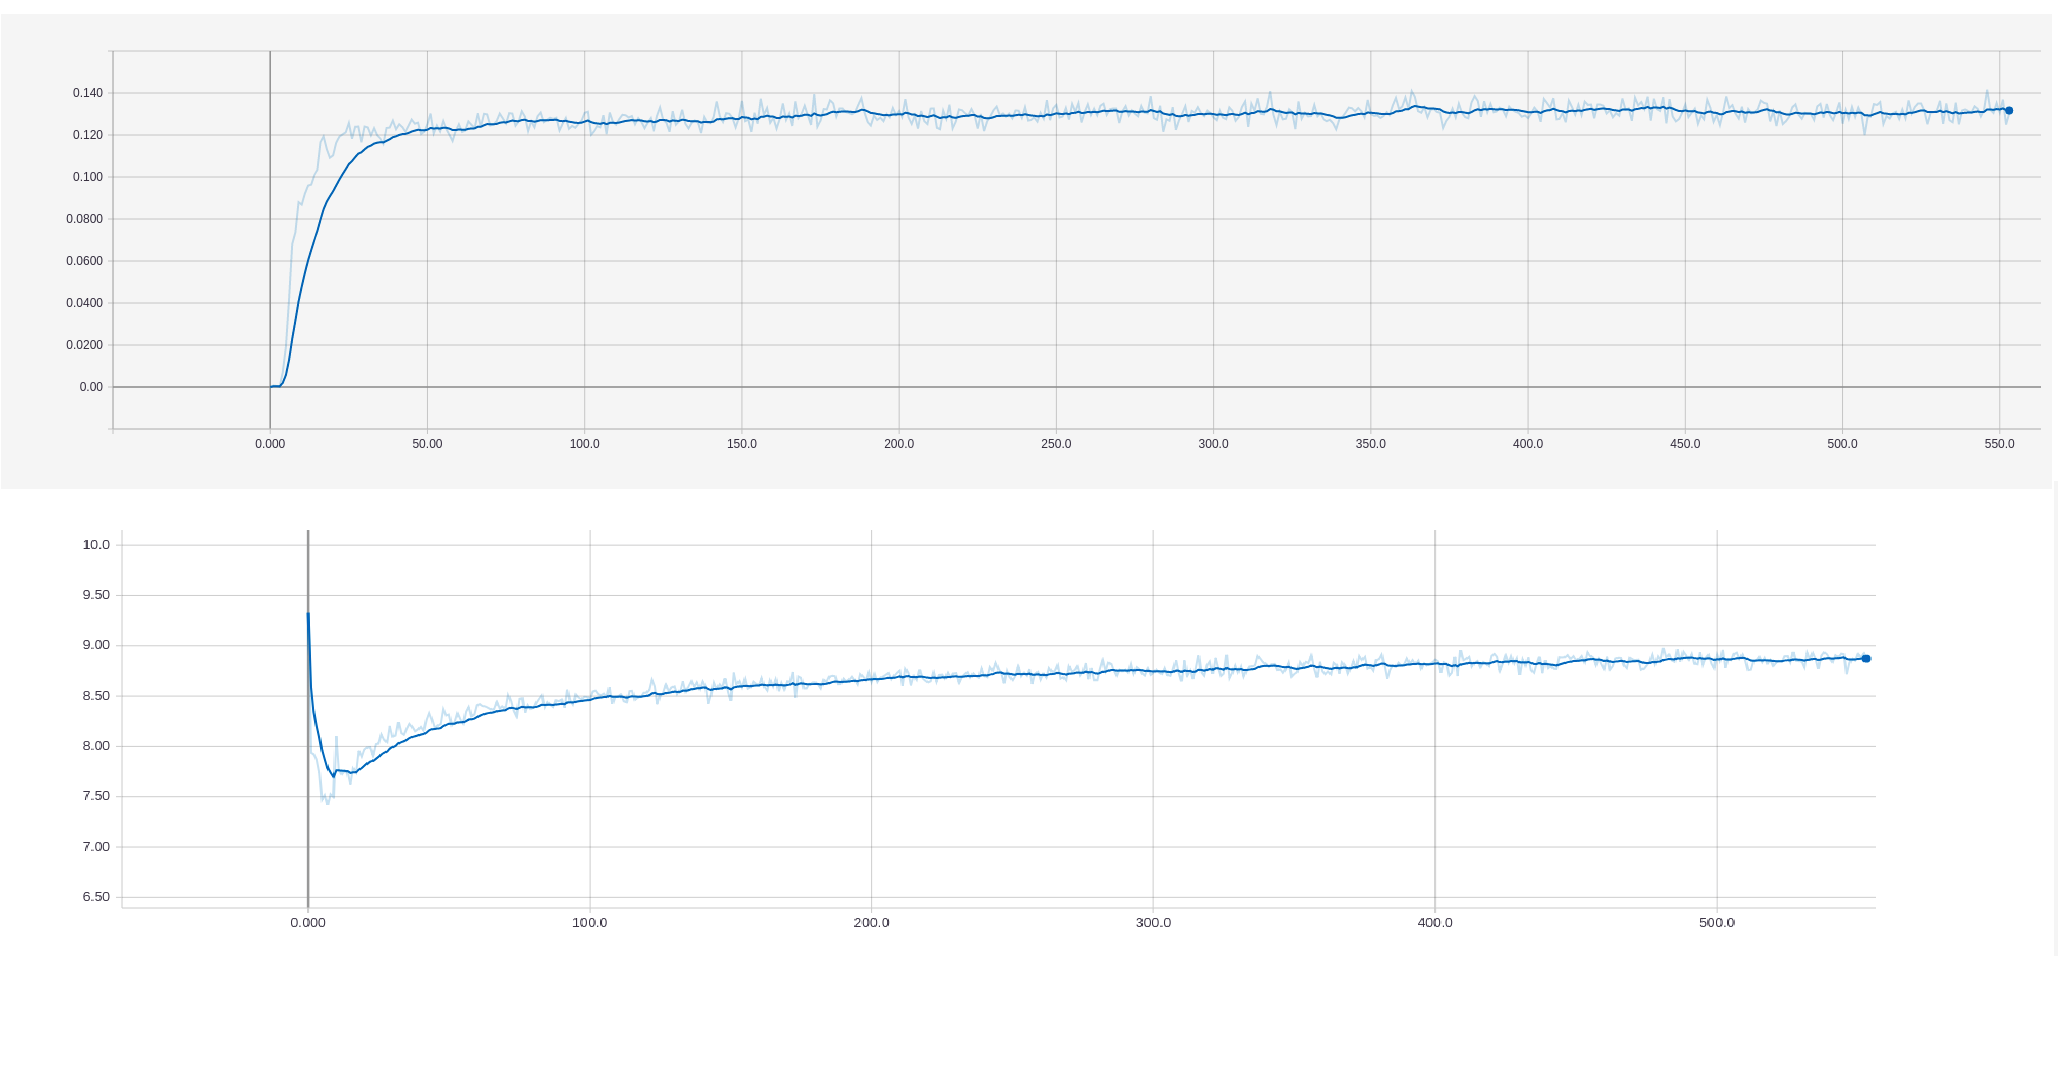
\includegraphics[scale=0.18]{figures/learning_curve.png}
    \caption{Accuracy and loss learning curves}
    \label{fig:edge_based_learning_curve_accuracy}
\end{figure}

\begin{figure}[h!]
    \centering
    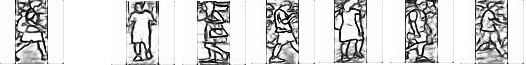
\includegraphics[scale=0.7]{figures/missclassifications.png}
    \caption{Typical miss-classifications}
    \label{fig:missclassifications}
\end{figure}

\subsubsection{Skeleton-based method}

The following table provides the results of the five independent runs of the Skeleton-based algorithm.

\begin{figure}[h!]
    \centering
    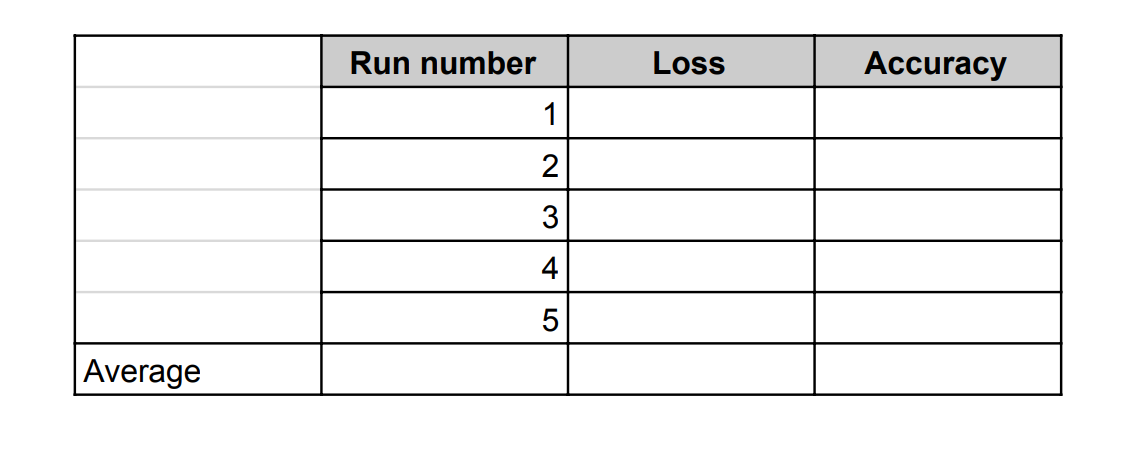
\includegraphics[scale=0.22]{figures/results.png}
    \caption{Results of five runs of the Edge-based algorithm}
    \label{fig:skeleton_based_met_results}
\end{figure}

\subsubsection{Combined method}

The following table provides the results of the five independent runs of the Edge-based algorithm.

\begin{figure}[h!]
    \centering
    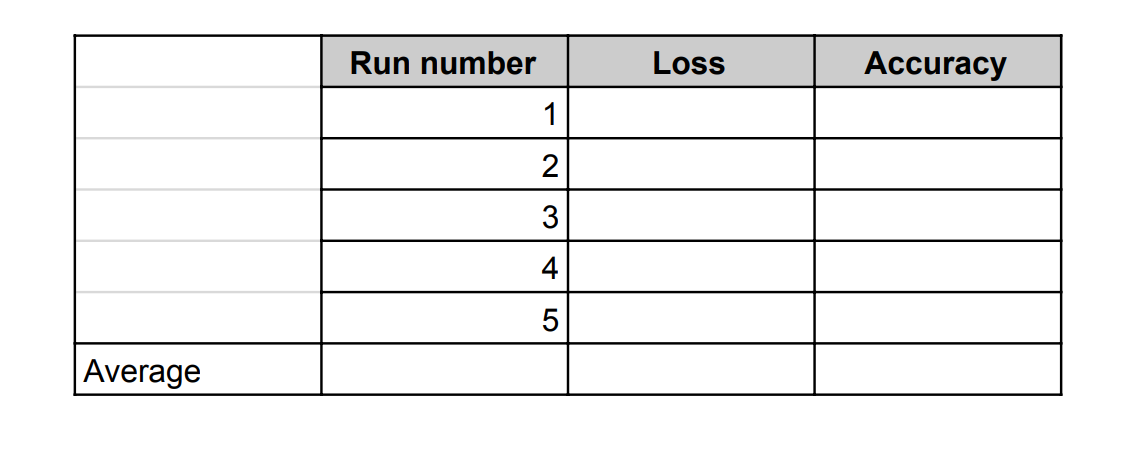
\includegraphics[scale=0.22]{figures/results.png}
    \caption{Results of five runs of the Edge-based algorithm}
    \label{fig:combined_met_results}
\end{figure}

Figures \ref{fig:combined_met_results} shows the Accuracy resp. Loss learning curve for the Combined method. The x-axis represents the number of iterations of the algorithm and the y-axis denotes the accuracy resp. loss.

\begin{figure}[h!]
    \centering
    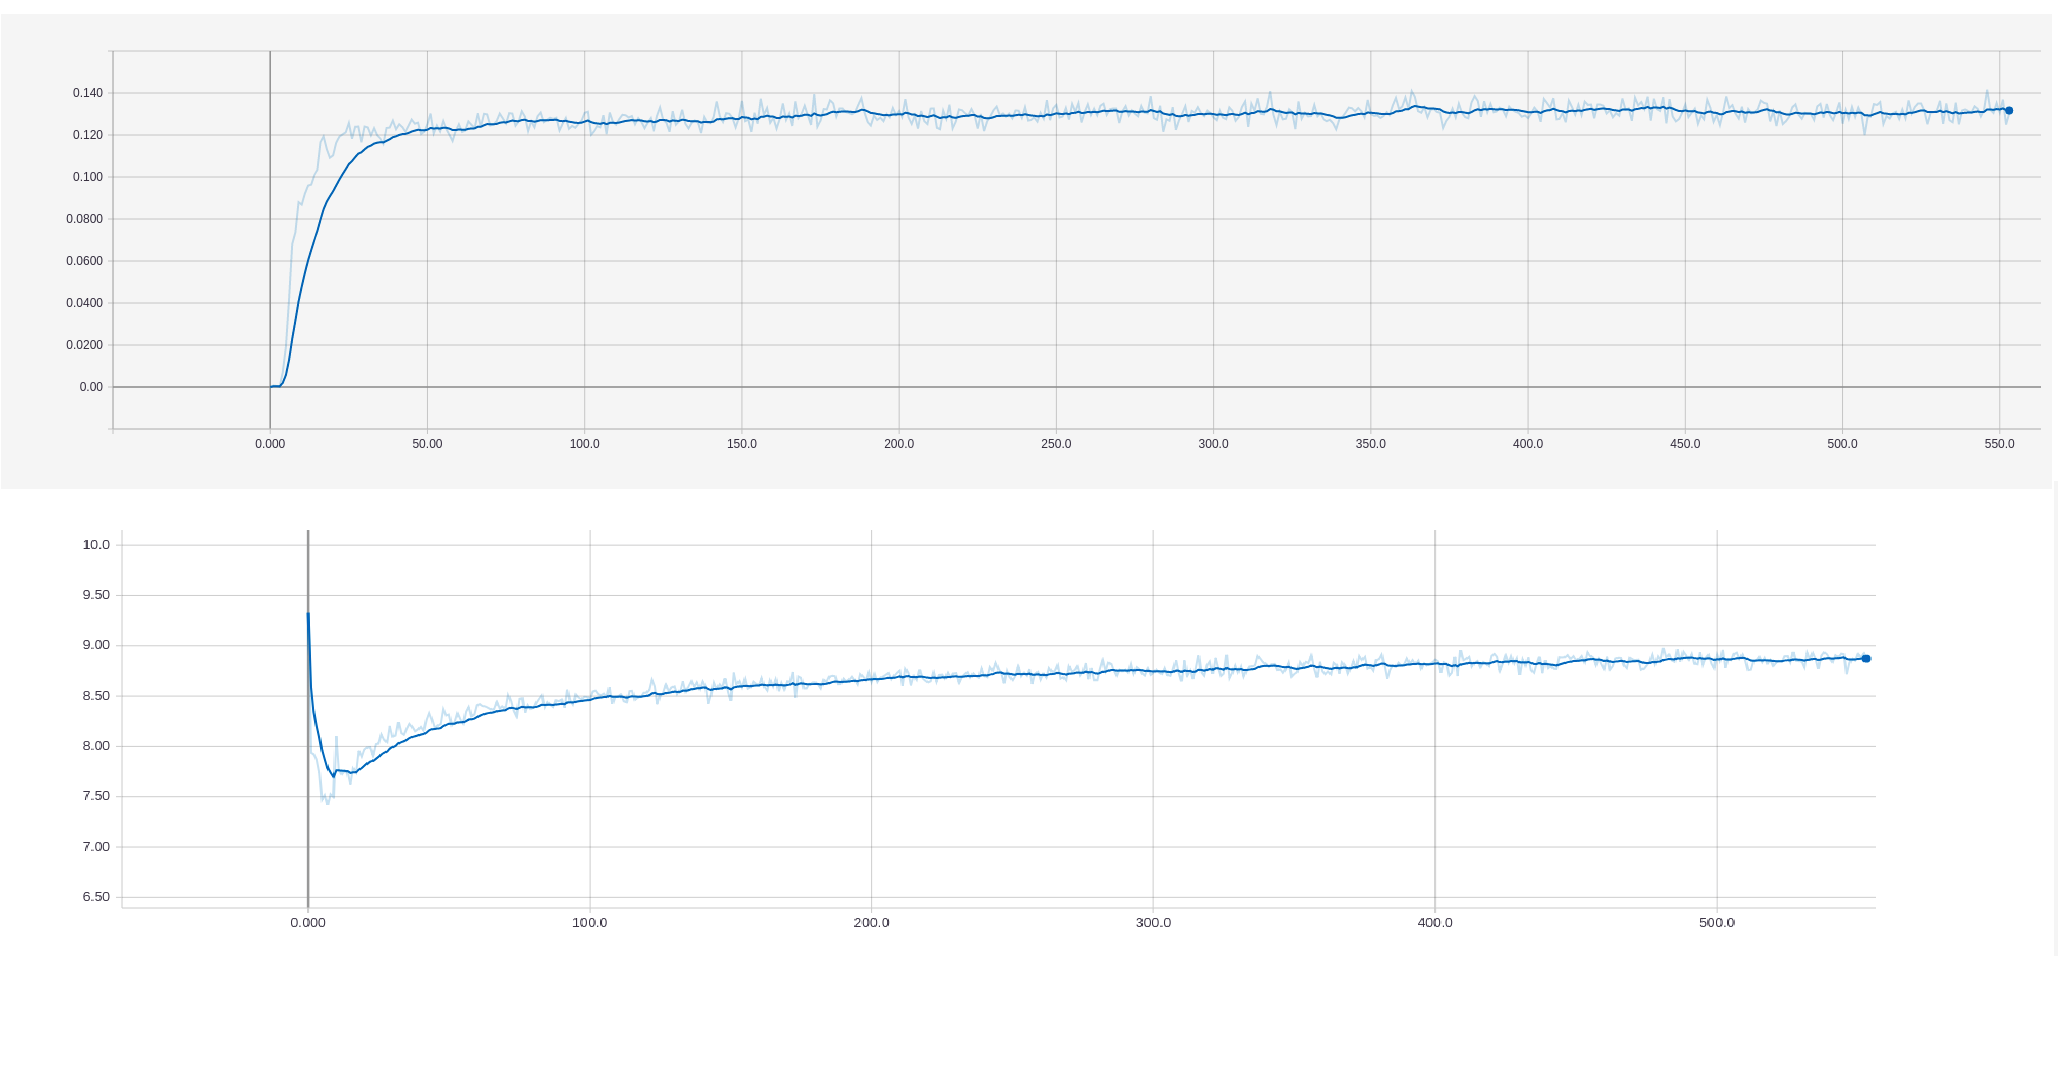
\includegraphics[scale=0.18]{figures/learning_curve.png}
    \caption{Accuracy and loss learning curves}
    \label{fig:edge_based_learning_curve_accuracy}
\end{figure}
\chapter{Future Work} \label{ch:results}
\chapter{Conclusion} \label{ch:conclusion}








% 

\chapter{Detailed results of the experiments} \label{app:exp_res}

The following tables contain more complete results of the experiments described in \cref{ch:exp}.

\begin{table}[h]
\begin{tabular}{r||c|c|c|c|c}
\toprule
& \multicolumn{5}{c}{Relative amounts of training data} \\
&          1 &       0.75 &        0.5 &       0.25 &      0.125 \\
\midrule
0   &  87.160835 &  87.914632 &  85.092499 &  80.308195 &  69.227414 \\
1   &  88.223817 &  87.523094 &  86.423896 &  80.806657 &  71.161864 \\
2   &  87.807642 &  86.651873 &  86.996770 &  83.227470 &  71.298274 \\
3   &  88.207577 &  88.134526 &  86.752232 &  79.188221 &  72.445672 \\
4   &  87.947029 &  88.178198 &  86.602650 &  80.259772 &  70.791102 \\
\midrule
5   &  87.938089 &  87.058472 &  83.267818 &  82.513815 &  68.779007 \\
6   &  88.187609 &  87.406726 &  87.131258 &  80.458106 &  73.018356 \\
7   &  88.056997 &  88.213705 &  87.196342 &  79.690593 &  66.413281 \\
8   &  87.692025 &  88.361035 &  86.544611 &  80.874767 &  70.388140 \\
9   &  88.000813 &  87.304882 &  86.577849 &  81.171910 &  65.811565 \\
\hline
\textbf{avg} &  87.922243 &  87.674714 &  86.258593 &  80.849951 &  69.933468 \\
\hline
\textbf{std} &   0.302300 &   0.542363 &   1.142954 &   1.158793 &   2.266158 \\
\bottomrule
\end{tabular}

\caption[All measured accuracies using supervised ULMFiT]{Accuracies measured in the experiment described in \cref{sec:expt1}}
\label{tab:exp1_complete}
\end{table}


\begin{table}[h]
\begin{tabular}{r||c|c|c|c|c}
\toprule
& \multicolumn{5}{c}{Relative amounts of training data} \\
&          1 &       0.75 &        0.5 &       0.25 &      0.125 \\
\midrule
0   &  87.160835 &  87.383913 &  85.794978 &  83.668693 &  81.707504 \\
1   &  88.223817 &  87.916595 &  86.762542 &  85.688351 &  80.610170 \\
2   &  87.807642 &  87.178675 &  86.570723 &  84.768064 &  80.977576 \\
3   &  88.207577 &  87.462209 &  87.182601 &  83.416468 &  82.076774 \\
4   &  87.947029 &  87.265326 &  86.869639 &  85.731833 &  80.338175 \\
\midrule
5   &  87.938089 &  87.383855 &  87.165173 &  84.760113 &  81.144016 \\
6   &  88.187609 &  87.307489 &  86.673243 &  83.840033 &  82.111950 \\
7   &  88.056997 &  88.248552 &  87.508883 &  84.917638 &  80.923438 \\
8   &  87.692025 &  87.362567 &  86.841745 &  85.943018 &  83.100916 \\
9   &  88.000813 &  86.971771 &  87.763805 &  84.733168 &  82.226157 \\
\hline
\textbf{avg} &  87.922243 &  87.448095 &  86.913333 &  84.746738 &  81.521668 \\
\hline
\textbf{std} &   0.302300 &   0.350518 &   0.516665 &   0.840956 &   0.819113 \\
\bottomrule
\end{tabular}

\caption[All measured accuracies using semi-supervised ULMFiT]{Accuracies measured in the experiment described in \cref{sec:expt2}}
\end{table}

\begin{table}[h]
    \centering
    \begin{tabular}{r||c|c|c|c|c}
    \toprule
    & \multicolumn{5}{c}{Relative amounts of training data} \\
    Class &      1 &      0.75 &      0.5 &      0.25 &      0.125 \\
    \midrule
    \textbf{alt.atheism}            &  19.56 &  21.57 &  24.33 &  37.05 &  46.58 \\
    comp.graphics            &  17.74 &  17.28 &  17.22 &  19.28 &  17.02 \\
    comp.os.ms-windows.misc  &  23.05 &  22.89 &  22.39 &  21.78 &  20.00 \\
    comp.sys.ibm.pc.hardware &  21.17 &  18.57 &  20.66 &  14.80 &  17.96 \\
    \textbf{comp.sys.mac.hardware}    &  13.45 &  16.52 &  16.52 &  26.130 &  30.75 \\
    \textbf{comp.windows.x  }         &  17.81 &  17.40 &  20.51 &  26.28 &  34.59 \\
    \textbf{misc.forsale }            &   9.28 &  10.92 &  12.92 &  23.74 &  29.74 \\
    rec.autos                &  10.68 &   9.06 &  11.59 &   8.41 &  11.19 \\
    \textbf{rec.motorcycles }         &   4.72 &   6.98 &   6.83 &  10.20 &  15.27 \\
    rec.sport.baseball       &   4.84 &   4.53 &   4.84 &   4.53 &   4.94 \\
    \hline
    rec.sport.hockey         &   1.80 &   2.01 &   1.80 &   1.95 &   2.41 \\
    sci.crypt                &   7.12 &   6.01 &   6.26 &   5.51 &   6.41 \\
    \textbf{sci.electronics}          &  19.03 &  18.02 &  22.39 &  31.55 &  37.86 \\
    \textbf{sci.med}                  &   8.74 &  10.05 &  11.21 &  17.68 &  22.58 \\
    \textbf{sci.space}                &   7.21 &   6.60 &   7.06 &  12.64 &  17.46 \\
    \textbf{soc.religion.christian}   &   7.19 &   7.69 &   8.54 &  14.82 &  19.35 \\
    \textbf{talk.politics.guns}       &  10.88 &  10.33 &  13.46 &  16.32 &  18.74 \\
    talk.politics.mideast    &  11.91 &  13.94 &  11.65 &  12.02 &  11.06 \\
    talk.politics.misc       &  38.77 &  37.55 &  37.10 &  36.57 &  37.75 \\
    talk.religion.misc       &  27.57 &  23.98 &  28.05 &  21.99 &  23.51 \\
    \bottomrule
    \end{tabular}
    \caption[Class errors with 10 classes unbalanced]{Average error per class with 10 classes unbalanced (in \textbf{bold}) as described in \cref{sec:expt3}.}
\end{table}{}

\begin{table}[h ]
    \centering
    \begin{tabular}{r||c|c|c|c|c}
    \toprule
    & \multicolumn{5}{c}{Relative amounts of training data} \\
    Class &      1 &      0.75 &      0.5 &      0.25 &      0.125 \\
    \midrule
    alt.atheism              &  19.56 &  20.50 &  20.25 &  24.51 &  20.94 \\
    comp.graphics            &  17.74 &  17.53 &  16.97 &  17.38 &  18.82 \\
    comp.os.ms-windows.misc  &  23.05 &  23.60 &  23.25 &  28.78 &  24.98 \\
    comp.sys.ibm.pc.hardware &  21.17 &  17.91 &  20.61 &  18.11 &  20.41 \\
    comp.sys.mac.hardware    &  13.45 &  15.27 &  15.58 &  15.64 &  14.70 \\
    \textbf{comp.windows.x  }         &  17.81 &  17.19 &  18.52 &  25.92 &  30.92 \\
    misc.forsale             &   9.28 &   9.85 &   8.51 &   8.46 &   8.72 \\
    rec.autos                &  10.68 &   8.71 &   9.11 &   9.52 &   9.72 \\
    rec.motorcycles          &   4.72 &   4.77 &   6.33 &   5.38 &   5.43 \\
    rec.sport.baseball       &   4.84 &   4.74 &   5.29 &   4.28 &   5.39 \\
    \hline
    rec.sport.hockey         &   1.80 &   1.55 &   1.70 &   1.90 &   1.65 \\
    sci.crypt                &   7.12 &   5.91 &   5.91 &   5.30 &   6.46 \\
    sci.electronics          &  19.03 &  18.12 &  17.71 &  16.69 &  15.27 \\
    sci.med                  &   8.74 &  10.40 &   8.54 &   8.99 &   8.69 \\
    sci.space                &   7.21 &   6.29 &   7.92 &   6.75 &   6.65 \\
    \textbf{soc.religion.christian}   &   7.19 &   6.68 &   9.05 &  13.37 &  22.06 \\
    talk.politics.guns       &  10.88 &  10.16 &   8.74 &   8.35 &   6.65 \\
    talk.politics.mideast    &  11.91 &  12.23 &  11.91 &  11.06 &   9.89 \\
    talk.politics.misc       &  38.77 &  37.42 &  36.97 &  39.61 &  39.61 \\
    talk.religion.misc       &  27.57 &  25.98 &  25.42 &  24.06 &  27.17 \\
    \bottomrule
    \end{tabular}
    \caption[Class errors with 10 classes unbalanced]{Average error per class with 2 classes unbalanced (in \textbf{bold}) as described in \cref{sec:expt4}.}
\end{table}{}


\chapter{Contents of the CD}



\dirtree{%
.1 /.
.2 src.
.3 model\_structure.
.3 scripts.
.3 fastai\_scripts.
.3 fresh\_models.
.3 notebooks\DTcomment{Jupyter notebooks used for data evaluation}.
.3 experiments\DTcomment{Files generated during the experiments}.
.4 exp1.
.4 exp2.
.4 exp3.
.4 exp4.
.2 thesis\DTcomment{\LaTeX  codes of this thesis}.
.3 figures.
.3 chapters.
}

\appendix



\bibliographystyle{plain}
\bibliography{bibliography}


\end{document}